\documentclass[11pt]{amsart}

\usepackage[letterpaper,margin=1.15in]{geometry}
\usepackage[T1]{fontenc}
\usepackage{lmodern}
\usepackage{microtype}
\usepackage{amsmath,amssymb,amsthm,mathtools}
\usepackage{graphicx}
\usepackage{booktabs}
\usepackage{enumitem}
\usepackage{alltt}
\usepackage{needspace}
\usepackage{xcolor}
\usepackage[colorlinks=true,linkcolor={blue!50!black},citecolor={blue!50!black},urlcolor={blue!50!black}]{hyperref}
\usepackage[capitalize,nameinlink]{cleveref}
\raggedbottom
\makeatletter
% With \raggedbottom every page has zero badness, so any negative penalty attracts the page break.
% The default \@secpenalty (-300) and the \penalty-100 inside \needspace both end pages early;
% this \needspace breaks only when less than #1 remains on the page.
\@secpenalty=0
\renewcommand{\needspace}[1]{\par\begingroup\setlength{\dimen@}{#1}%
  \dimen@ii\pagegoal \advance\dimen@ii-\pagetotal
  \ifdim\dimen@>\dimen@ii \ifdim\dimen@ii>\z@\vfil\fi\penalty-\@M\fi\endgroup}
\makeatother
\renewcommand{\topfraction}{0.85}
\renewcommand{\bottomfraction}{0.6}
\renewcommand{\textfraction}{0.1}
\renewcommand{\floatpagefraction}{0.75}

% ------------------------------------------------------------------ theorem environments
\newtheorem{thm}{Theorem}[section]
\newtheorem{prop}[thm]{Proposition}
\newtheorem{lem}[thm]{Lemma}
\newtheorem{cor}[thm]{Corollary}
\theoremstyle{definition}
\newtheorem{defn}[thm]{Definition}
\newtheorem{rem}[thm]{Remark}
\numberwithin{equation}{section}
\numberwithin{figure}{section}
\numberwithin{table}{section}
\crefname{thm}{Theorem}{Theorems}
\crefname{prop}{Proposition}{Propositions}
\crefname{lem}{Lemma}{Lemmas}
\crefname{cor}{Corollary}{Corollaries}
\crefname{defn}{Definition}{Definitions}
\crefname{rem}{Remark}{Remarks}

% ------------------------------------------------------------------ notation
\newcommand{\R}{\mathbb{R}}
\newcommand{\Z}{\mathbb{Z}}
\newcommand{\Lh}{L_{\mathrm{horiz}}}
\newcommand{\Lv}{L_{\mathrm{vert}}}
\newcommand{\lamstar}{\lambda^{*}}
\newcommand{\muA}{\mu_{\mathrm{A}}}
\newcommand{\muZ}{\mu_{\mathrm{Z}}}
\newcommand{\muR}{\mu_{\mathrm{R}}}
\newcommand{\bu}{\mathbf{u}}
\newcommand{\bv}{\mathbf{v}}
\newcommand{\bw}{\mathbf{w}}
\newcommand{\Lo}{\mathit{Lo}}
\newcommand{\Up}{\mathit{Up}}
\newcommand{\Tmain}{\tfrac{353}{200}}
\newcommand{\dg}{^{\circ}}
\newcommand{\pos}[1]{(#1)_{+}}
\DeclareMathOperator{\diam}{diam}

% abstract set as in the article class: centred bold heading above an indented block
\makeatletter
\renewenvironment{abstract}{%
  \global\setbox\abstractbox=\vtop \bgroup
    \normalfont\Small
    \list{}{\labelwidth\z@ \leftmargin3pc \rightmargin\leftmargin
      \listparindent\normalparindent \itemindent\z@ \parsep\z@ \@plus\p@
      \let\fullwidthdisplay\relax}%
    \item\relax{\centering\bfseries\abstractname\par}\vskip0.5\baselineskip
    \ignorespaces
}{%
  \endlist\egroup
  \ifx\@setabstract\relax \@setabstracta \fi
}
\makeatother

\begin{document}

\title[The ambidextrous moving sofa problem]{Upper bounds for the\\ ambidextrous moving sofa problem}

\author{Devin O'Keefe}
\address{Independent Researcher}
\email{okeefede@tcd.ie}

\subjclass[2020]{Primary 49Q10; Secondary 52A10, 68V05, 68V20}
\keywords{moving sofa problem, ambidextrous sofa, computer-assisted proof, branch and bound, exact arithmetic, formal verification, Lean}

\begin{abstract}
The ambidextrous moving sofa problem asks for the largest area of a connected planar shape that can be moved around a right-angled corner in a hallway of unit width, both to the left and to the right, from the same starting position. The largest known such shape, found numerically by Gibbs and derived exactly by Romik, has area $1.64495521\ldots$. We prove with computer assistance that every ambidextrous sofa has area at most $353/200=1.765$, and give a computer-free proof of the bound $2\sqrt{2}-1=1.8284\ldots$. Both proofs control the orientation of the sofa by a variant of an argument of Gerver, as modified by Baek, that does not assume monotone rotation. The proofs are formalised in Lean, apart from the run of the verified checker on the certificate.
\end{abstract}

\maketitle

\section{Introduction}\label{sec:intro}

\subsection{The problem}

Leo Moser's moving sofa problem \cite{moser1966} asks for the planar shape of largest area that can be moved around a right-angled corner in a hallway of unit width. This paper is about a variant in which the shape must be able to take the corner in either direction:

\begin{quote}
\itshape What is the largest area of a connected planar shape that can be moved around such a corner both when it turns to the left and when it turns to the right, starting in both cases from the same position?
\end{quote}

\noindent Following Romik \cite{romik2018}, we call such a shape an \emph{ambidextrous sofa}, and write $\muA$ for the supremum of their areas. The common starting position (\cref{fig:problem}(a)) distinguishes the problem from the ordinary one: without it, every shape that can take the corner to the right could also take it to the left (\cref{rem:definitions}(3)). Formal definitions are in \cref{sec:definitions}.

\begin{figure}[t]
\centering
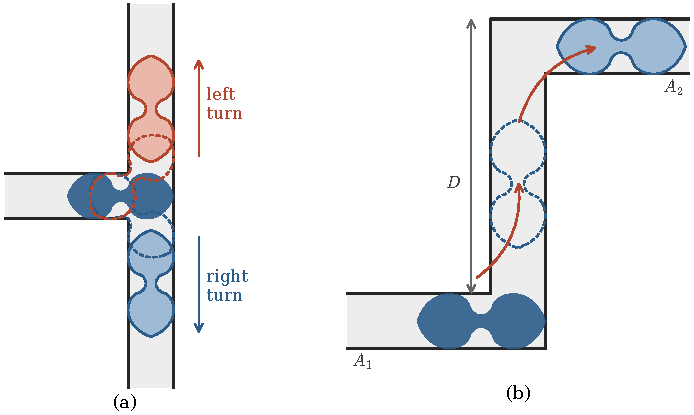
\includegraphics[width=\textwidth]{figures/fig_problem.pdf}
\caption{(a) The hallway turning right (downward) and the hallway turning left (upward), drawn together. Romik's shape $\Sigma$ is shown in its common starting position (dark), halfway through each turn (dashed), and after each turn (light). (b) The same shape passing through the Z-shaped corridor $Z_D$ of \cref{sec:zcorridor}: at the start, in the vertical section, and at the end (drawn with $D=5$).}
\label{fig:problem}
\end{figure}

The ordinary, one-sided problem has a long history \cite{croft1991,romik2018,wagner1976}. The upper bound $2\sqrt{2}\approx 2.8284$ and a shape of area $\pi/2+2/\pi\approx 2.2074$ go back to Hammersley \cite{hammersley1968}. Gerver \cite{gerver1992} found a slightly larger shape, of area $2.21953166\ldots$, and conjectured that it is optimal. Kallus and Romik \cite{kallusromik2018} lowered the upper bound to $2.37$ with a computer-assisted proof; their method is our starting point. Baek \cite{baek2024} has announced a proof that Gerver's shape is optimal, which has since been formalised in the Lean proof assistant \cite{cureton2026movingsofa,cao2026sofaformal}.

Variants of the problem with other corridors were already discussed in the 1960s; see \cite[Section~1.2]{romik2018} and \cite{wagner1976}. For the ambidextrous problem, Gibbs \cite{gibbs2014} numerically computed a shape of area about $1.64495$, and Romik \cite{romik2018} derived it exactly. This shape $\Sigma$, shown in \cref{fig:problem}, is symmetric under reflection in the midline of the hallway, and its area is
\[
\muR \;=\; \sqrt[3]{3+2\sqrt{2}}+\sqrt[3]{3-2\sqrt{2}}-1+\arctan\Big[\tfrac12\Big(\sqrt[3]{\sqrt2+1}-\sqrt[3]{\sqrt2-1}\Big)\Big] \;=\; 1.64495521\ldots,
\]
with the arctangent in radians. Romik obtained $\Sigma$ from conditions that a shape of maximal area can be expected to satisfy, and it is a natural candidate for the solution \cite{romik2018,kallusromik2018}. Whether it is optimal remains open. Determining $\muA$ is Problem~6.63 in the list of Georgiev, G\'omez-Serrano, Tao and Wagner \cite{georgiev2025alphaevolve} and Problem C41b in the list of optimisation constants maintained by Davis, Ivanisvili, Tao and others \cite{optimisation-constants-repo}.

Much less is known about upper bounds. Every ambidextrous sofa is an ordinary sofa, so upper bounds for the ordinary problem apply. Kallus and Romik point this out for their bound $2.37$ and call the gap between the bounds ``an appealing opportunity for further work'' \cite[Section~5]{kallusromik2018}. Granting Baek's theorem, the inherited bound becomes $2.2195\ldots$. Recently, Bonfioli \cite{bonfioli2026} announced the bound $2\sqrt2-1$, using a relaxation of the kind described in \cref{sec:45}. \Cref{tab:history} summarises the bounds.

\begin{table}[t]
\centering
\caption{Bounds on the ambidextrous sofa constant $\muA$.}
\label{tab:history}
\begin{tabular}{@{}llll@{}}
\toprule
 & Bound & Source & Status \\
\midrule
Lower & $1.64495$ & Gibbs \cite{gibbs2014} & numerical \\
      & $\muR=1.64495521\ldots$ & Romik \cite{romik2018} & proved \\
\midrule
Upper & $2\sqrt2 = 2.8284\ldots$ & Hammersley \cite{hammersley1968} & proved \\
      & $2.37$ & Kallus--Romik \cite{kallusromik2018} & proved, computer-assisted \\
      & $2.2195\ldots$ & Baek \cite{baek2024} & preprint \\
      & $2\sqrt2-1 = 1.8284\ldots$ & Bonfioli \cite{bonfioli2026} & preprint \\
      & $2\sqrt2-1 = 1.8284\ldots$ & \cref{thm:hand} & proved \\
      & $\Tmain = 1.765$ & \cref{thm:main} & proved, computer-assisted \\
\bottomrule
\end{tabular}
\end{table}

\needspace{7\baselineskip}
\subsection{Results}

We prove two upper bounds. Besides the formulation above, we treat a second formulation \cite{optimisation-constants-repo}, in which the sofa travels through a Z-shaped corridor $Z_D$: a left turn followed by a right turn into a horizontal arm at height $D$ above the first (\cref{fig:problem}(b)).

\begin{thm}[Main theorem]\label{thm:main}
Every ambidextrous sofa has area at most $\Tmain=1.765$. Moreover, for every $D\ge 7$, every sofa that can be moved through the Z-shaped corridor $Z_D$ has area at most $\Tmain$.
\end{thm}

Together with Romik's shape, this gives
\[
1.64495521\ldots \;\le\; \muA \;\le\; 1.765 .
\]

The computer is used only for a single explicit inequality (\cref{thm:computation}).

\begin{thm}[A bound without computer assistance]\label{thm:hand}
Every ambidextrous sofa has area at most $2\sqrt2-1=1.8284\ldots$, and so does every sofa that can be moved through $Z_D$ for some $D\ge 7$.
\end{thm}

\Cref{thm:hand} is weaker than \cref{thm:main}, but its proof is self-contained and uses no computer. The bound was announced by Bonfioli \cite{bonfioli2026}, whose proof also intersects the horizontal strip with one hallway of each handedness at $45\dg$. The note describes each motion by a rotation path on $[0\dg,90\dg]$, which assumes that the sofa passes through the orientation $45\dg$ in each turn; \cref{prop:natural} shows that every sofa of area greater than $\sqrt2$ does so.

Both theorems are formalised in Lean (\cref{sec:lean}), using the definitions of the moving sofa problem from the Formal Conjectures project \cite{formalconjectures} and the definition of ambidextrous sofas proposed in \cite{fc_pr6424}. For \cref{thm:hand} the formal proof is complete; for \cref{thm:main} it covers everything except the run of the checker on the certificate, which is done by compiled code.

\subsection{The idea of the proofs}

We follow the approach of Kallus and Romik \cite{kallusromik2018}. In the frame of the sofa, the hallway moves around it, so the sofa lies in every position that the hallway takes. Intersect finitely many of these positions with the horizontal strip in which the sofa starts; since the sofa is connected, it lies in a single connected component of this intersection. Now forget the motion and let the translations of the positions vary independently. The area of the sofa is at most the supremum, over all translations, of the largest area of a connected component of such an intersection. Kallus and Romik bounded suprema of this kind by computer.

An ambidextrous sofa has two motions, and hence two families of hallway positions: rotated copies of the hallway that turns right and of its mirror image, the hallway that turns left (\cref{fig:hallways}). A single rotated hallway from each family already gives the bound $2\sqrt2-1$, whereas a single rotated hallway in the ordinary problem gives only Hammersley's $2\sqrt2$.

To use a hallway rotated by an angle $a$, one needs to know that at some moment of its turn the sofa is rotated by $a$ in the direction of the turn. In the ordinary problem, Kallus and Romik rely on Gerver's theorem \cite[Theorem~1]{gerver1992} that a sofa of maximal area can be moved with monotonically increasing rotation, so that every orientation up to the final one is visited. No such result is known for ambidextrous sofas, and a priori a sofa might wobble, rotate the wrong way first, or rotate by more than a full turn.

We avoid the issue with a variant of an argument that Baek \cite[Theorem~1.5.1]{baek2024} gives for the ordinary problem, as a modification of an argument of Gerver \cite[p.~271]{gerver1992}. Suppose that at some moment the sofa is rotated by $45\dg$ against the direction of its turn, or by $135\dg$ with it. Seen from the sofa, the hallway then meets every horizontal line in a segment of length exactly $\sqrt2$ (\cref{lem:sideways} and \cref{fig:45}(a)), and since the sofa also lies in a horizontal strip of width $1$, its area is at most $\sqrt2$. So a sofa of area greater than $\sqrt2$ never reaches these orientations. At the end of the turn the sofa lies in the outgoing arm, a vertical strip of width $1$. Seen from the sofa, this strip makes an angle of $90\dg-\theta_1$ with the horizontal strip in which the sofa started, where $\theta_1$ is the final orientation. Two nonparallel strips of width $1$ whose directions make an angle $\varphi$ meet in area $1/|\sin\varphi|$, so the area $\lambda(S)$ of the sofa is at most $1/|\cos\theta_1|$ (\cref{lem:strips}). Hence $\theta_1$ is within $\arcsin(1/\lambda(S))$ of an odd multiple of $90\dg$. Since the forbidden orientations cannot be crossed, it is close to $90\dg$ in the direction of the turn. The intermediate value theorem then shows that during each turn the sofa passes through every orientation from $0\dg$ to $\arccos(1/\lambda(S))$ in the direction of the turn; for area $1.765$ this is about $55\dg$ (\cref{prop:natural}). Nothing about the motion is assumed except continuity.

In the Z-shaped corridor both turns happen during a single motion. A short additional argument (\cref{sec:zproof}) shows that when $D\ge7$ a sofa of area greater than $\sqrt2$ is too short to be in both corners at once, which again yields hallways from both families.

With one angle, $45\dg$, from each family, the optimisation problem can be solved by hand: its value is exactly $2\sqrt2-1$ (\cref{prop:onehalf}), attained by the configuration in \cref{fig:45}(b). This proves \cref{thm:hand}.

For \cref{thm:main} we use two angles from each family, $\arcsin(3/5)\approx 36.87\dg$ and $\arcsin(4/5)\approx 53.13\dg$, and bound the optimisation problem by computer. These angles have rational sines and cosines, so the whole computation can be done in exact rational arithmetic. The eight unknown translation parameters can be restricted to a bounded box. A floating-point search divides this box into smaller boxes and records the subdivision as a \emph{certificate}, and a separate checker verifies in exact arithmetic that the objective is at most $\Tmain$ on every box. Errors in the search cannot affect the result, since they can only produce a certificate that the checker rejects. The main checker is written and proved correct in Lean; checkers written in C and in Python also accept the certificate (\cref{sec:computation}).

\section{Definitions}\label{sec:definitions}

\subsection{Notation}

We work in the plane $\R^2$ with coordinates $(x,y)$. Angles are measured in degrees, counterclockwise, and $R_\theta$ denotes rotation about the origin by $\theta$. A \emph{rigid motion} is a map of the form $z\mapsto R_\theta z+\mathbf{x}$ with $\theta\in\R$ and $\mathbf{x}\in\R^2$. We write $\lambda$ for area (Lebesgue measure) and, following \cite{kallusromik2018}, $\lamstar(X)$ for the supremum of the areas of the connected components of a closed set $X\subset\R^2$, with $\lamstar(\emptyset)=0$; the components are closed, so their areas are defined. If $X\subset Y$ are closed then $\lamstar(X)\le\lamstar(Y)$, because every connected component of $X$ lies in a component of $Y$. For a real number $r$ we write $\pos{r}=\max(r,0)$.

The hallways are built from the horizontal and vertical strips
\[
H=\R\times[0,1], \qquad V=[0,1]\times\R .
\]
As in \cite{kallusromik2018,romik2018}, let
\[
\Lh=(-\infty,1]\times[0,1], \qquad \Lv=[0,1]\times(-\infty,1], \qquad L_0=\Lh\cup\Lv .
\]
The set $L_0$ is a hallway of unit width that comes in from the left and turns right, downward, at the unit square $[0,1]^2$. Let
\[
\rho(x,y)=(x,\,1-y)
\]
be the reflection in the midline $y=\tfrac12$ of $H$. It maps $\Lh$ to itself, and $\rho(L_0)=\Lh\cup\big([0,1]\times[0,\infty)\big)$ is the hallway that comes in from the left and turns left, upward (\cref{fig:problem}(a)).

\subsection{Sofas and motions}

\begin{defn}\label{def:sofa}
\leavevmode
\begin{enumerate}[label=(\alph*)]
\item A \emph{sofa} is a nonempty, closed, connected subset of $\R^2$.
\item A \emph{motion} is a pair of continuous functions $\theta\colon[0,1]\to\R$ and $\mathbf{x}\colon[0,1]\to\R^2$ with $\theta(0)=0$ and $\mathbf{x}(0)=0$. For a set $S$ we write $S_t=R_{\theta(t)}S+\mathbf{x}(t)$ for its position at time $t$, and call $\theta(t)$ its \emph{orientation}.
\item A sofa $S$ \emph{turns right} if $S\subset\Lh$ and there is a motion such that $S_t\subset L_0$ for all $t\in[0,1]$ and $S_1\subset\Lv$. It \emph{turns left} if $S\subset\Lh$ and there is a motion such that $S_t\subset\rho(L_0)$ for all $t$ and $S_1\subset\rho(\Lv)$.
\item A sofa is \emph{ambidextrous} if it turns right and turns left. The two motions may differ, but both start from the same position $S\subset\Lh$.
\item The \emph{ambidextrous sofa constant} is $\muA=\sup\{\lambda(S): S \text{ is an ambidextrous sofa}\}$.
\end{enumerate}
\end{defn}

\begin{rem}\label{rem:definitions}
\leavevmode
\begin{enumerate}[label=(\arabic*),leftmargin=*]
\item Recording the orientation $\theta(t)$ as a real number, rather than as an angle modulo $360\dg$, loses no generality: every continuous path of rigid motions that starts at the identity lifts uniquely to a motion in our sense. The real-valued orientation lets us distinguish, for instance, a sofa that has turned by $-90\dg$ from one that has turned by $270\dg$.

\item Conjugating a motion by $\rho$ gives a motion whose orientation is $-\theta(t)$. Hence a sofa $S$ turns left if and only if its mirror image $\rho(S)$ turns right, and $S$ is ambidextrous if and only if both $S$ and $\rho(S)$ turn right. This is the notion used in a proposed formalisation in Lean \cite{fc_pr6424}.

\item If the two turns were allowed to start from different positions, the ambidextrous problem would coincide with the ordinary one, because every sofa that turns right also turns left \emph{from some starting position}.

To see this, suppose that a sofa $S$ turns right with the motion $t\mapsto S_t$, and let $\chi(x,y)=(y,x)$ be the reflection that swaps $\Lh$ and $\Lv$ and maps $L_0$ to itself. Running the motion backwards and reflecting it gives the positions $t\mapsto\chi(S_{1-t})$. They form a motion of the mirror image $\chi(S_1)$ of $S$, with orientation $\theta(1)-\theta(1-t)$, which starts in $\Lh$, stays in $L_0$ and ends in $\Lv$. So $\chi(S_1)$ turns right, and by~(2) the set $\rho\chi(S_1)$ turns left. As $\rho\chi$ is a rotation followed by a translation, so is the map that takes $S$ to $\rho\chi(S_1)$.

The documentation of \cite{fc_pr6424} makes the same point. The statement of Problem~6.63 in \cite{georgiev2025alphaevolve} leaves the requirement of a common starting position implicit.

\item Romik's shape $\Sigma$ is ambidextrous \cite[Theorem~5]{romik2018}. Hence $\muA\ge\muR=1.64495521\ldots$.
\end{enumerate}
\end{rem}

\subsection{The Z-shaped corridor}\label{sec:zcorridor}

Another formulation \cite{optimisation-constants-repo} asks for the largest sofa that can travel through a corridor with a left turn followed by a right turn, the two turns being far apart. For $D>0$ let
\[
A_1=(-\infty,1]\times[0,1],\qquad M=[0,1]\times[0,D+1],\qquad A_2=[0,\infty)\times[D,D+1],
\]
and let $Z_D=A_1\cup M\cup A_2$. A sofa travelling to the right in $A_1$ turns left into the vertical section $M$, moves up, and turns right into $A_2$ (\cref{fig:problem}(b)).

\begin{defn}\label{def:z}
A sofa $S$ \emph{passes through} $Z_D$ if $S\subset A_1$ and there is a motion such that $S_t\subset Z_D$ for all $t\in[0,1]$ and $S_1\subset A_2$. We write $\muZ(D)$ for the supremum of the areas of such sofas.
\end{defn}

Romik's shape passes through $Z_D$ when $D$ is large enough. It can make the first turn with its left-turning motion, which ends with the shape rotated by exactly $90\dg$ and lying in the vertical arm. The second turn is a right turn seen in a rotated frame. The rigid motion $\Phi(z)=R_{90\dg}z+(1,D)$ maps $L_0$ onto the hallway
\[
\Phi(L_0)=\big([0,1]\times(-\infty,D+1]\big)\cup A_2
\]
around the upper corner. So the shape can slide up the strip $[0,1]\times\R$ to the position $\Phi(\Sigma)$ and then follow the positions $\Phi(\Sigma_t)$, where $t\mapsto\Sigma_t$ is the right-turning motion of $\Sigma$. Since both motions stay in a bounded region, all positions lie in $Z_D$ once $D$ is large. Hence $\muZ(D)\ge\muR$ for all large $D$.

We do not know whether $\muZ(D)$ and $\muA$ are equal for large $D$. In the Z-shaped corridor the two turns start from different positions, and neither formulation obviously reduces to the other. Our upper bounds hold for both.

\subsection{Boundedness}

\Cref{def:sofa} does not require a sofa to be bounded, but every sofa that can make one of the moves above is.

\begin{lem}\label{lem:bounded}
Every sofa that turns right, turns left, or passes through $Z_D$ is bounded.
\end{lem}

\begin{proof}
Suppose $S$ is unbounded, and consider a motion as in the relevant definition. Since $S\subset\Lh$, we can choose points $p_n\in S$ with $|p_n|\to\infty$, and then $p_n/|p_n|\to(-1,0)$. Fix $t$. The points $q_n=R_{\theta(t)}p_n+\mathbf{x}(t)$ lie in $S_t$ and satisfy $q_n/|p_n|\to R_{\theta(t)}(-1,0)$. On the other hand, the only directions in which $L_0$ is unbounded are $(-1,0)$ and $(0,-1)$: if points $q_n\in L_0$ satisfy $|q_n|\to\infty$, then every limit of $q_n/|q_n|$ is one of these two vectors. For $\rho(L_0)$ the two directions are $(-1,0)$ and $(0,1)$, and for $Z_D$ they are $(-1,0)$ and $(1,0)$. In each case $R_{\theta(t)}(-1,0)$ must be one of two vectors for every $t$. As $\theta$ is continuous and $\theta(0)=0$, this forces $\theta(t)=0$ for all $t$. But the final position $S_1$ lies in $\Lv$, $\rho(\Lv)$ or $A_2$, which are unbounded only in the directions $(0,-1)$, $(0,1)$ and $(1,0)$ respectively, and none of these is $R_0(-1,0)$. This is a contradiction.
\end{proof}

\needspace{9\baselineskip}
\section{Hallway relaxations}\label{sec:relaxations}

\subsection{Rotated hallways}

For an angle $a\in\R$ let
\[
f_a(x,y)=x\cos a+y\sin a, \qquad g_a(x,y)=-x\sin a+y\cos a
\]
be the coordinates in a frame rotated by $a$, so that $R_{-a}z=(f_a(z),g_a(z))$. For $\bu=(u_1,u_2)\in\R^2$ we define the rotated and translated hallway
\begin{equation}\label{eq:La}
\begin{split}
L_a(\bu)&=R_a(\bu+L_0)\\
&=\{u_1\le f_a\le u_1+1,\ g_a\le u_2+1\}\cup\{f_a\le u_1+1,\ u_2\le g_a\le u_2+1\}.
\end{split}
\end{equation}
This is the notation of \cite{kallusromik2018}, except that $a$ may be any real angle, not only one between $0\dg$ and $90\dg$. We call the two sets in \eqref{eq:La} the \emph{arms} of the hallway: the first is the image of $\Lv$, the arm that leaves the corner, and the second the image of $\Lh$, the arm that leads into it. We also use the mirrored hallways $\rho(L_b(\bv))$; see \cref{fig:hallways}.

The next lemma describes the hallway in the frame of the sofa. In part~(ii) the mirrored hallway appears with the opposite angle, because $\rho$ reverses the sense of rotation: $\rho\circ R_\theta\circ\rho^{-1}$ is a rotation by $-\theta$ followed by a translation.

\needspace{5\baselineskip}
\begin{lem}[The hallway seen from the sofa]\label{lem:frame}
Let $S\subset\R^2$ and let $\Psi(z)=R_\theta z+\mathbf{x}$ be a rigid motion.
\begin{enumerate}[label=(\roman*)]
\item If $\Psi(S)\subset L_0$, then $S\subset L_{-\theta}(\bu)$ for some $\bu\in\R^2$.
\item If $\Psi(S)\subset\rho(L_0)$, then $S\subset\rho(L_{\theta}(\bv))$ for some $\bv\in\R^2$.
\item If $\Psi(S)\subset R_{90\dg}L_0+\mathbf{q}$ for some $\mathbf{q}\in\R^2$, then $S\subset L_{90\dg-\theta}(\bu)$ for some $\bu\in\R^2$.
\end{enumerate}
\end{lem}

\begin{proof}
In each case $S\subset \Psi^{-1}(Y)=R_{-\theta}(Y-\mathbf{x})$, where $Y$ is the hallway in question. For (i), $R_{-\theta}(L_0-\mathbf{x})=L_{-\theta}(-\mathbf{x})$.

\needspace{9\baselineskip}
For (ii), separate the reflection $\rho$ into its linear part and a translation: $\rho(z)=\sigma z+e_2$, where $\sigma(x,y)=(x,-y)$ and $e_2=(0,1)$. Put $\mathbf{w}=\sigma(e_2-\mathbf{x})$, so that $\rho(L_0)-\mathbf{x}=\sigma(L_0+\mathbf{w})$. Using $R_{-\theta}\sigma=\sigma R_\theta$, we get
\begin{align*}
R_{-\theta}\big(\rho(L_0)-\mathbf{x}\big)&=\sigma R_\theta(L_0+\mathbf{w})=\sigma\big(L_\theta(\mathbf{w})\big)=\rho\big(L_\theta(\mathbf{w})\big)-e_2\\
&=\rho\big(L_\theta(\mathbf{w})+e_2\big)=\rho\big(L_\theta(\mathbf{w}+R_{-\theta}e_2)\big).
\end{align*}
In the second line we used that $\rho(Y)-e_2=\rho(Y+e_2)$ for every set $Y$, and that $R_\theta(L_0+\mathbf{w})+e_2=R_\theta(L_0+\mathbf{w}+R_{-\theta}e_2)$. Hence $S\subset\rho\big(L_\theta(\bv)\big)$ with $\bv=\mathbf{w}+R_{-\theta}e_2$.

For (iii), $R_{-\theta}(R_{90\dg}L_0+\mathbf{q}-\mathbf{x})=R_{90\dg-\theta}\big(L_0+R_{-90\dg}(\mathbf{q}-\mathbf{x})\big)=L_{90\dg-\theta}\big(R_{-90\dg}(\mathbf{q}-\mathbf{x})\big)$.
\end{proof}

Thus a sofa that has rotated clockwise by $a$ during a right turn (so $\theta=-a$) lies in a hallway $L_a(\bu)$, and one that has rotated counterclockwise by $b$ during a left turn lies in a mirrored hallway $\rho(L_b(\bv))$. Romik's shape rotates monotonically by $90\dg$ in both turns, so for it these angles fill $[0\dg,90\dg]$. A general motion need not reach them all; \cref{sec:reduction} shows which ones every sofa of large area must reach.


\needspace{8\baselineskip}
\begin{figure}[h]
\centering
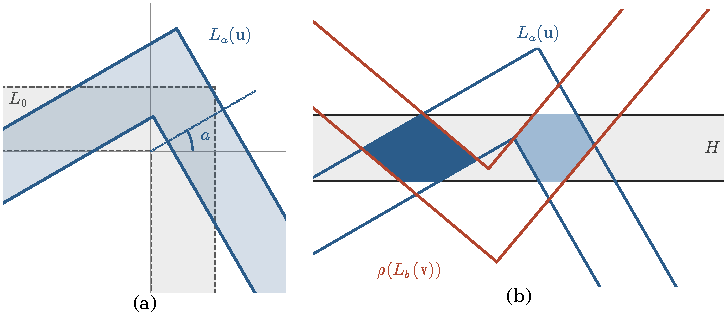
\includegraphics[width=0.9\textwidth]{figures/fig_hallways.pdf}
\caption{(a) The hallway $L_0$ (dashed) and the rotated and translated hallway $L_a(\bu)$ for $a=30\dg$. (b) A hallway $L_a(\bu)$ with $a=30\dg$ and a mirrored hallway $\rho(L_b(\bv))$ with $b=40\dg$. Their intersection with the strip $H$ has two connected components, of areas $1.005$ (dark) and $0.859$ (light); the value of $\lamstar$ is the larger one.}
\label{fig:hallways}
\end{figure}

\subsection{The relaxation}

\begin{defn}\label{def:G}
For finite sets $A,B\subset\R$ of angles let
\begin{equation}\label{eq:G}
G(A;B)=\sup\,\lamstar\Big(H\cap\bigcap_{a\in A}L_a(\bu_a)\cap\bigcap_{b\in B}\rho\big(L_b(\bv_b)\big)\Big),
\end{equation}
where the supremum is over all choices of vectors $\bu_a,\bv_b\in\R^2$.
\end{defn}

When $B=\emptyset$ and $A\subset(0\dg,90\dg)$, this is the quantity $G_{\boldsymbol\alpha}$ of Kallus and Romik \cite{kallusromik2018}. The sets $A$ and $B$ correspond to the right turn and the left turn.

\begin{lem}\label{lem:relax}
Let $S\subset H$ be closed and connected. If $S\subset L_a(\bu_a)$ for every $a\in A$ and $S\subset\rho(L_b(\bv_b))$ for every $b\in B$, then $\lambda(S)\le G(A;B)$.
\end{lem}

\begin{proof}
$S$ is a connected subset of the intersection in \eqref{eq:G}, so it lies in a single connected component of it.
\end{proof}

We also need two simple estimates. The first underlies the angle conditions in \cref{sec:reduction}.

\begin{lem}[Two strips]\label{lem:strips}
Let $S\subset H$ be measurable and let $\Psi(z)=R_\theta z+\mathbf{x}$ be a rigid motion.
\begin{enumerate}[label=(\roman*)]
\item If $\Psi(S)\subset V$, then $\lambda(S)\le 1/|\cos\theta|$.
\item If $\Psi(S)$ lies in a horizontal strip $\R\times[c,c+1]$, then $\lambda(S)\le1/|\sin\theta|$.
\end{enumerate}
Here $1/0=\infty$.
\end{lem}

\begin{proof}
In case (i), $S$ lies in the intersection of $H$ with the strip $\Psi^{-1}(V)$, also of width $1$, whose direction makes an angle of $90\dg-\theta$ with the horizontal. Two strips of width $1$ whose directions make an angle $\varphi$ with $\sin\varphi\neq0$ intersect in a parallelogram of area $1/|\sin\varphi|$. For $\varphi=90\dg-\theta$ we have $|\sin\varphi|=|\cos\theta|$, and if $\cos\theta=0$ there is nothing to prove. Case (ii) is the same with the angle $-\theta$.
\end{proof}

\needspace{8\baselineskip}
The second estimate bounds the length of a connected set that fits in a rotated hallway and in $H$.

\begin{lem}[Width]\label{lem:width}
Let $0\dg<a<90\dg$, write $c=\cos a$ and $s=\sin a$, and let
\[
W_a=\frac{1+s}{c}+\frac{1+c}{s}.
\]
If $K$ is a connected subset of $H\cap L_a(\bu)$ or of $H\cap\rho(L_a(\bu))$, then the projection of $K$ to the $x$-axis is an interval of length at most $W_a$. Consequently $\diam K\le\sqrt{W_a^2+1}$.
\end{lem}

\begin{proof}
Since $\rho$ preserves $H$ and $x$-coordinates, it suffices to treat $L_a(\bu)$. Let $0\le y\le1$. A point $(x,y)$ of the first arm satisfies $u_1\le xc+ys\le u_1+1$, so $x$ lies in the interval $[(u_1-s)/c,\,(u_1+1)/c]$ of length $(1+s)/c$. A point of the second arm satisfies $u_2\le -xs+yc\le u_2+1$, so $x$ lies in $[(-u_2-1)/s,\,(c-u_2)/s]$, of length $(1+c)/s$. The projection of $K$ is connected, hence an interval, and it is contained in the union of these two intervals; so its length is at most the sum of their lengths.
\end{proof}

For example, $W_{45\dg}=2+2\sqrt2$, and $W_a=5$ for $a=\arcsin(3/5)$ and $a=\arcsin(4/5)$.

\subsection{Hallways at \texorpdfstring{$45\dg$}{45 degrees}}\label{sec:45}

We need two facts about hallways rotated by odd multiples of $45\dg$: \cref{lem:sideways}, which is used for both theorems, and \cref{prop:onehalf}, which gives \cref{thm:hand}. We say that the corner of $L_0$ points in the direction $45\dg$, the direction of the vector from its inner corner $(0,0)$ to its outer corner $(1,1)$. Hence the corner of $L_a(\bu)$ points in the direction $a+45\dg$, and that of $\rho(L_b(\bv))$ in the direction $-(b+45\dg)$. The first fact concerns the four cases in which the corner points horizontally, so that the hallway lies ``sideways'' across $H$ (\cref{fig:45}(a)).

\begin{figure}[h]
\centering
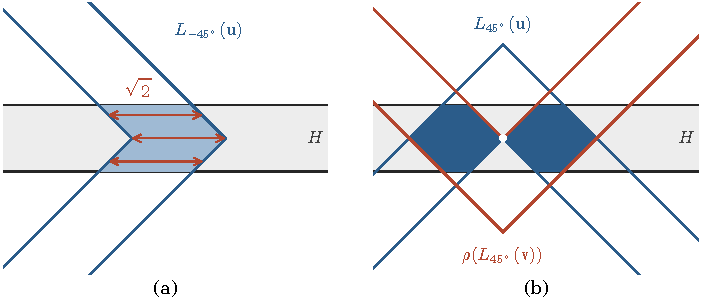
\includegraphics[width=\textwidth]{figures/fig_45.pdf}
\caption{Hallways at $45\dg$. (a) A sideways hallway $L_{-45\dg}(\bu)$. Every horizontal line meets it in a segment of length $\sqrt2$, so it meets $H$ in area exactly $\sqrt2$ (\cref{lem:sideways}). (b) The extremal configuration of \cref{prop:onehalf}: for $\bu=\bv=(0,1/\sqrt2)$ the set $H\cap L_{45\dg}(\bu)\cap\rho(L_{45\dg}(\bv))$ consists of two squares of side $1$, each cut off by $H$, which touch at the point $(-\tfrac12,\tfrac12)$. Its area is $2\sqrt2-1$.}
\label{fig:45}
\end{figure}


\needspace{7\baselineskip}
\begin{lem}[Sideways hallways]\label{lem:sideways}
Let $X$ be one of $L_{-45\dg}(\bu)$, $L_{135\dg}(\bu)$, $\rho(L_{-45\dg}(\bu))$ and $\rho(L_{135\dg}(\bu))$, for some $\bu\in\R^2$. Then every horizontal line meets $X$ in a segment of length exactly $\sqrt2$. Consequently $\lambda(H\cap X)=\sqrt2$, and every measurable set $S\subset H\cap X$ has $\lambda(S)\le\sqrt2$.
\end{lem}

\begin{proof}
First let $X=L_{-45\dg}(\bu)$. Then $f=(x-y)/\sqrt2$ and $g=(x+y)/\sqrt2$, and by \eqref{eq:La}
\[
X=\{f\le u_1+1,\ g\le u_2+1\}\setminus\{f<u_1,\ g<u_2\}.
\]
On the horizontal line at height $y$, both $f$ and $g$ increase with $x$ at rate $1/\sqrt2$. Put $\xi_1=\sqrt2\,u_1+y$ and $\xi_2=\sqrt2\,u_2-y$. The first set above meets the line in the points with $x\le\min(\xi_1,\xi_2)+\sqrt2$, and the removed set in the points with $x<\min(\xi_1,\xi_2)$. So the line meets $X$ in the segment $x_0\le x\le x_0+\sqrt2$ with $x_0=\min(\xi_1,\xi_2)$.

The other three cases follow, because $L_{135\dg}(\bu)=R_{180\dg}L_{-45\dg}(\bu)$ and both the rotation $R_{180\dg}$ and the reflection $\rho$ map horizontal lines to horizontal lines without changing lengths. Integrating the length $\sqrt2$ over $0\le y\le1$ gives $\lambda(H\cap X)=\sqrt2$.
\end{proof}

The second fact is that the relaxation with one angle, $45\dg$, on each side can be computed exactly.

\begin{prop}[One angle on each side]\label{prop:onehalf}
For all $\bu,\bv\in\R^2$,
\[
\lambda\big(H\cap L_{45\dg}(\bu)\cap\rho(L_{45\dg}(\bv))\big)\le 2\sqrt2-1,
\]
with equality when $\bu=\bv=(0,1/\sqrt2)$, in which case the set is connected. In particular $G(\{45\dg\};\{45\dg\})=2\sqrt2-1$.
\end{prop}

The proof, an exact computation of areas by slicing along horizontal lines, is in \cref{app:onehalf}. For comparison, with the hallway $L_{45\dg}(\bu)$ alone the supremum of $\lamstar$ is $2\sqrt2$: this is Hammersley's bound, written in the language of relaxations \cite[Section~2]{kallusromik2018}, and it comes from the two arms of $L_{45\dg}(\bu)$, each of which meets $H$ inside a parallelogram of area $\sqrt2$. \Cref{fig:45}(b) shows the effect of the mirrored hallway in the extremal configuration: it cuts each arm down to a unit square. A unit square tilted by $45\dg$ meets $H$ in area at most $\sqrt2-\tfrac12$, and both squares attain this, so the total is $2\sqrt2-1$, exactly $1$ less than Hammersley's bound.

\section{From motions to a single relaxation}\label{sec:reduction}

We show that a sofa of large area lies in an intersection of hallways as in \cref{def:G}, for suitable angle sets $A$ and $B$, so that its area is at most $G(A;B)$. When we say that a sofa turns right, turns left or passes through $Z_D$, we fix a motion as in \cref{def:sofa} or \cref{def:z} and write $\theta(t)$ and $S_t$ for its orientation and positions. Throughout, $T>\sqrt2$ is a threshold, and we write
\[
\delta_T=\arcsin(1/T), \qquad \gamma_T=\arccos(1/T)=90\dg-\delta_T .
\]
Since $T>\sqrt2$ we have $\delta_T<45\dg<\gamma_T$. \Cref{lem:strips} explains the role of $\delta_T$: a sofa $S\subset H$ of area greater than $T$ can be moved into a vertical strip of width $1$ only when its orientation is within $\delta_T$ of an odd multiple of $90\dg$, and into a horizontal one only when it is within $\delta_T$ of a multiple of $180\dg$.

\needspace{10\baselineskip}
\subsection{Two hallways}\label{sec:twocorridors}

\begin{lem}[No sideways turn]\label{lem:noside}
Let $S$ be a sofa with $\lambda(S)>\sqrt2$, and let $(\theta,\mathbf{x})$ be a motion.
\begin{enumerate}[label=(\roman*)]
\item If the motion moves $S$ around the right turn as in \cref{def:sofa}(c), then $-135\dg<\theta(t)<45\dg$ for all $t$.
\item If the motion moves $S$ around the left turn, then $-45\dg<\theta(t)<135\dg$ for all $t$.
\end{enumerate}
\end{lem}

\begin{proof}
(i) For every $t$ we have $S_t\subset L_0$, so $S\subset L_{-\theta(t)}(\bu)$ for some $\bu$ by \cref{lem:frame}(i); also $S\subset\Lh\subset H$. If $\theta(t)$ were equal to $45\dg$ modulo $180\dg$, the hallway $L_{-\theta(t)}(\bu)$ would be $L_{-45\dg}(\bu)$ or $L_{135\dg}(\bu)$, and \cref{lem:sideways} would give $\lambda(S)\le\sqrt2$. So $\theta$ never takes a value in $45\dg+180\dg\Z$. Since $\theta$ is continuous and $\theta(0)=0$, it stays strictly between the two neighbouring values $-135\dg$ and $45\dg$.

(ii) The same argument with \cref{lem:frame}(ii) excludes the values in $-45\dg+180\dg\Z$.
\end{proof}

\begin{prop}[Turning the right way]\label{prop:natural}
Let $T>\sqrt2$ and let $S$ be a sofa with $\lambda(S)>T$.
\begin{enumerate}[label=(\roman*)]
\item If $S$ turns right, then for every $a\in[0\dg,\gamma_T]$ there is $\bu\in\R^2$ with $S\subset L_a(\bu)$.
\item If $S$ turns left, then for every $b\in[0\dg,\gamma_T]$ there is $\bv\in\R^2$ with $S\subset\rho(L_b(\bv))$.
\end{enumerate}
\end{prop}

\begin{proof}
(i) At the end of the motion $S_1\subset\Lv\subset V$, while $S\subset H$. By \cref{lem:strips}(i), $|\cos\theta(1)|\le1/\lambda(S)<1/T=\sin\delta_T$, so $\theta(1)$ lies within $\delta_T$ of an odd multiple of $90\dg$. By \cref{lem:noside}(i), $\theta(1)$ also lies in $(-135\dg,45\dg)$. Since $\delta_T<45\dg$, the only possibility is $-90\dg-\delta_T<\theta(1)<-90\dg+\delta_T$, and in particular $\theta(1)<-\gamma_T$. As $\theta(0)=0$, the intermediate value theorem gives, for every $a\in[0\dg,\gamma_T]$, a time $t$ with $\theta(t)=-a$, and then $S\subset L_a(\bu)$ for some $\bu$ by \cref{lem:frame}(i).

(ii) In the same way, \cref{lem:strips}(i) and \cref{lem:noside}(ii) give $90\dg-\delta_T<\theta(1)<90\dg+\delta_T$. So $\theta$ takes every value $b\in[0\dg,\gamma_T]$, and \cref{lem:frame}(ii) gives $S\subset\rho(L_b(\bv))$.
\end{proof}

\Cref{lem:noside,prop:natural} are a variant of an argument of Gerver \cite[p.~271]{gerver1992}, in the form given by Baek \cite[Theorem~1.5.1]{baek2024}, who uses it to show that a moving sofa of area at least $2.2$ admits a motion that rotates by at least $\sec^{-1}(2.2)\approx63\dg$. The argument uses only the continuity of the motion and its final position; no monotonicity is assumed. In the ordinary problem, where the areas of interest are about $2.2$, it gives hallways $L_a(\bu)$ only for angles $a$ up to about $63\dg$; the relaxations of \cite{kallusromik2018} also use larger angles, and for these Kallus and Romik rely on Gerver's theorem.

\begin{thm}[Reduction for two hallways]\label{thm:reduction2}
Let $T>\sqrt2$, and let $A,B\subset[0\dg,\gamma_T]$ be finite. Then every ambidextrous sofa $S$ satisfies $\lambda(S)\le\max\{T,\,G(A;B)\}$. Hence $\muA\le\max\{T,G(A;B)\}$.
\end{thm}

\begin{proof}
If $\lambda(S)>T$, then by \cref{prop:natural} $S$ lies in a hallway $L_a(\bu_a)$ for each $a\in A$ and in a mirrored hallway $\rho(L_b(\bv_b))$ for each $b\in B$. Since also $S\subset\Lh\subset H$, \cref{lem:relax} gives $\lambda(S)\le G(A;B)$.
\end{proof}

\subsection{The Z-shaped corridor}\label{sec:zproof}

In the corridor $Z_D$ the sofa first turns left, around the lower corner, and then right, around the upper corner. The two turns happen during a single motion, and a priori the sofa might be in both corners at once, or begin one turn before it has finished the other. We rule this out by showing that a sofa of area greater than $\sqrt2$ is shorter than the vertical section of the corridor. We use two regions of $Z_D$ (\cref{fig:zproof}(a)):
\[
\Lo=Z_D\cap\{y\le D-\tfrac12\}, \qquad \Up=Z_D\cap\{y\ge\tfrac32\}.
\]
For $D\ge2$ they overlap in the rectangle $\Lo\cap\Up=[0,1]\times[\frac32,D-\frac12]$ of the vertical section, and
\begin{equation}\label{eq:LoUp}
\Lo\subset\rho(L_0), \qquad \Up\subset R_{90\dg}L_0+(1,D),
\end{equation}
since $R_{90\dg}L_0+(1,D)=\big([0,1]\times(-\infty,D+1]\big)\cup\big([0,\infty)\times[D,D+1]\big)$.

\begin{figure}[t]
\centering
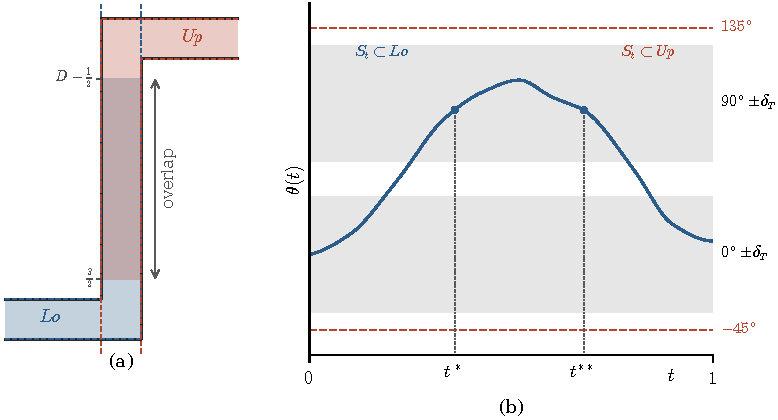
\includegraphics[width=\textwidth]{figures/fig_zproof.pdf}
\caption{(a) The corridor $Z_D$ (here $D=7$) with its lower region $\Lo$ and its upper region $\Up$. The dashed lines show the hallways $\rho(L_0)$ and $R_{90\dg}L_0+(1,D)$ that contain them. (b) A schematic picture of the orientation $\theta(t)$ of a sofa of area greater than $T$ passing through $Z_D$. The orientation never reaches $-45\dg$ or $135\dg$. At the times $t^*$ and $t^{**}$ of \cref{thm:reductionZ} the sofa lies in the overlap of $\Lo$ and $\Up$, so its orientation is within $\delta_T$ of $90\dg$ there; the grey bands have half-width $\delta_T$ for $T=\Tmain$.}
\label{fig:zproof}
\end{figure}

\needspace{10\baselineskip}
\begin{lem}[No sideways position in $Z_D$]\label{lem:zside}
Every line $x+y=c$ meets $Z_D$ in a segment of length $\sqrt2$. Consequently, if a sofa $S$ with $\lambda(S)>\sqrt2$ passes through $Z_D$ with the motion $(\theta,\mathbf{x})$, then $-45\dg<\theta(t)<135\dg$ for all $t$.
\end{lem}

\begin{proof}
A direct check shows that the projection to the $x$-axis of the intersection of $Z_D$ with the line $x+y=c$ is $[c-1,c]$ if $c\le1$, $[0,1]$ if $1\le c\le D+1$, and $[c-D-1,c-D]$ if $c\ge D+1$. In each case the intersection is a segment of length $\sqrt2$.

Now suppose that $\theta(t)$ equals $-45\dg$ modulo $180\dg$ for some $t$. Then $S\subset H\cap R_{-\theta(t)}(Z_D-\mathbf{x}(t))$. The rigid motion $z\mapsto R_{\theta(t)}z+\mathbf{x}(t)$ maps horizontal lines to lines of slope $-1$, so every horizontal line meets $R_{-\theta(t)}(Z_D-\mathbf{x}(t))$ in a segment of length $\sqrt2$, and hence $\lambda(S)\le\sqrt2$, a contradiction. By continuity, $\theta$ stays between $-45\dg$ and $135\dg$.
\end{proof}

\needspace{6\baselineskip}
\begin{lem}[A sofa of area greater than $\sqrt2$ is short]\label{lem:diameter}
Let $D\ge4$. If a sofa $S$ with $\lambda(S)>\sqrt2$ passes through $Z_D$, then $\diam S<5$.
\end{lem}

\begin{proof}
The idea is that the sofa must reach orientation $45\dg$ while it is still in the lower region, and at that moment it lies in a hallway $\rho(L_{45\dg}(\bv))$, which forces it to be short by \cref{lem:width}.

By \cref{lem:bounded}, $S$ is compact. The set of times $t$ with $S_t\subset\Lo$ is closed and contains $0$. Let $\tau$ be the largest time such that $S_t\subset\Lo$ for all $t\in[0,\tau]$. Then $\tau<1$, since $S_1\subset A_2$ is disjoint from $\Lo$. The maximum height $h(t)$ of the points of $S_t$ depends continuously on $t$, because $S$ is compact. Therefore $h(\tau)=D-\frac12$: otherwise $h(t)<D-\frac12$ for all $t$ near $\tau$, and then $S_t\subset Z_D\cap\{y<D-\frac12\}\subset\Lo$ for all $t$ slightly larger than $\tau$.

We claim that $\theta(\tau)\ge45\dg$. Suppose instead that $\theta(\tau)<45\dg$; then $-45\dg<\theta(\tau)<45\dg$ by \cref{lem:zside}. The set $S_\tau$ lies in the strip $R_{\theta(\tau)}H+\mathbf{x}(\tau)$, of width $1$, whose direction makes an angle of less than $45\dg$ with the horizontal. Above the interval $0\le x\le1$, this strip spans a range of heights of length at most $1/\cos\theta(\tau)+|\tan\theta(\tau)|<\sqrt2+1$. Since $S_\tau$ contains a point at height $D-\frac12>1$, and such points of $\Lo$ have $0\le x\le 1$, every point of the strip above $[0,1]$ has height greater than $D-\frac12-(\sqrt2+1)>1$, using $D\ge4$.

Thus the strip avoids the unit square $[0,1]^2$. Now $\Lo$ is the union of $A_1$ and $[0,1]\times[0,D-\frac12]$, and these two sets meet only in $[0,1]^2$. So $S_\tau$ is contained in the union of two disjoint closed sets, one inside $A_1$ and one inside $[0,1]\times[0,D-\frac12]$. Since $S_\tau$ is connected and contains a point of height $D-\frac12$, it lies in the second set, and hence in $V$. Now \cref{lem:strips}(i) gives $\lambda(S)\le1/\cos\theta(\tau)<\sqrt2$, a contradiction.

So $\theta(\tau)\ge45\dg$, and by the intermediate value theorem $\theta(t_0)=45\dg$ for some $t_0\in[0,\tau]$. As $S_{t_0}\subset\Lo\subset\rho(L_0)$, \cref{lem:frame}(ii) gives $S\subset H\cap\rho(L_{45\dg}(\bv))$ for some $\bv$. By \cref{lem:width}, $\diam S\le\sqrt{W_{45\dg}^2+1}=\sqrt{13+8\sqrt2}<5$.
\end{proof}

\begin{lem}[One corner at a time]\label{lem:onecorner}
Let $D\ge7$, and let $S$ be a sofa with $\lambda(S)>\sqrt2$ that passes through $Z_D$. Then at every time $t$, either $S_t\subset\Lo$ or $S_t\subset\Up$.
\end{lem}

\begin{proof}
By \cref{lem:diameter}, $\diam S_t<5\le D-2$. So $S_t$ cannot contain both a point of height less than $\frac32$ and a point of height greater than $D-\frac12$. If $S_t$ has no point above height $D-\frac12$, it lies in $\Lo$. Otherwise it has no point below height $\frac32$, and it lies in $\Up$.
\end{proof}

The constant $7$ is not optimal: moving the thresholds $\frac32$ and $D-\frac12$ closer to $1$ and $D$ gives a slightly smaller value. We have not looked for the smallest $D$ for which the argument works.

\begin{thm}[Reduction for the Z-shaped corridor]\label{thm:reductionZ}
Let $T>\sqrt2$ and $D\ge7$, and let $A\subset[\delta_T,\gamma_T]$ and $B\subset[0\dg,\gamma_T]$ be finite. Then every sofa $S$ that passes through $Z_D$ satisfies $\lambda(S)\le\max\{T,G(A;B)\}$. Hence $\muZ(D)\le\max\{T,G(A;B)\}$.
\end{thm}

\begin{proof}
Suppose $\lambda(S)>T$. Let $\mathcal{T}_{\mathrm{lo}}$ and $\mathcal{T}_{\mathrm{up}}$ be the sets of times $t$ with $S_t\subset\Lo$ and $S_t\subset\Up$ respectively. Both are closed, their union is $[0,1]$ by \cref{lem:onecorner}, and $0\in\mathcal{T}_{\mathrm{lo}}\setminus\mathcal{T}_{\mathrm{up}}$, $1\in\mathcal{T}_{\mathrm{up}}\setminus\mathcal{T}_{\mathrm{lo}}$. Let $t^*$ be the smallest element of $\mathcal{T}_{\mathrm{up}}$ and $t^{**}$ the largest element of $\mathcal{T}_{\mathrm{lo}}$. Every time before $t^*$ lies in $\mathcal{T}_{\mathrm{lo}}$, and this set is closed, so $t^*\in\mathcal{T}_{\mathrm{lo}}$. In the same way $t^{**}\in\mathcal{T}_{\mathrm{up}}$. So at both times the sofa lies in $\Lo\cap\Up\subset V$.

By \cref{lem:strips}(i) and \cref{lem:zside}, $\theta(t^*)$ and $\theta(t^{**})$ lie within $\delta_T$ of $90\dg$. At the end, $S_1\subset A_2$ lies in a horizontal strip, so by \cref{lem:strips}(ii) and \cref{lem:zside}, $\theta(1)$ lies within $\delta_T$ of $0\dg$.

\emph{The left turn.} For $t\in[0,t^*]$ we have $S_t\subset\Lo\subset\rho(L_0)$ by \eqref{eq:LoUp}, so $S\subset\rho(L_{\theta(t)}(\bv))$ for some $\bv$ by \cref{lem:frame}(ii). Since $\theta(0)=0$ and $\theta(t^*)>90\dg-\delta_T=\gamma_T$, every $b\in[0\dg,\gamma_T]$ is a value of $\theta$ on $[0,t^*]$. So $S$ lies in a mirrored hallway $\rho(L_b(\bv_b))$ for every $b\in B$.

\emph{The right turn.} For $t\in[t^{**},1]$ we have $S_t\subset\Up\subset R_{90\dg}L_0+(1,D)$, so $S\subset L_{90\dg-\theta(t)}(\bu)$ for some $\bu$ by \cref{lem:frame}(iii). Since $\theta(t^{**})>90\dg-\delta_T$ and $\theta(1)<\delta_T$, the angle $90\dg-\theta(t)$ takes every value in $[\delta_T,\gamma_T]$ on $[t^{**},1]$. So $S$ lies in a hallway $L_a(\bu_a)$ for every $a\in A$.

Finally $S\subset A_1\subset H$, and \cref{lem:relax} gives $\lambda(S)\le G(A;B)$.
\end{proof}

The condition $A\subset[\delta_T,\gamma_T]$, rather than $A\subset[0\dg,\gamma_T]$, is needed because the right turn does not start from a known orientation: at the time $t^{**}$ we only know that $|90\dg-\theta(t^{**})|<\delta_T$, so angles in $[0\dg,\delta_T)$ need not be visited during the right turn. The upper limit $\gamma_T$ comes from the final orientation, as in \cref{thm:reduction2}.

\subsection{Proof of \texorpdfstring{\cref{thm:hand}}{Theorem 1.2}}\label{sec:proofhand}

Let $T=2\sqrt2-1>\sqrt2$, so that $\delta_T<45\dg<\gamma_T$. Taking $A=B=\{45\dg\}$ in \cref{thm:reduction2,thm:reductionZ}, and using $G(\{45\dg\};\{45\dg\})=2\sqrt2-1$ from \cref{prop:onehalf}, we obtain $\lambda(S)\le 2\sqrt2-1$ for every ambidextrous sofa and for every sofa that passes through $Z_D$ with $D\ge7$. \qed

\section{Bounding a relaxation by computer}\label{sec:method}

For more than one angle on each side we do not know how to evaluate $G(A;B)$ by hand, so we bound it by computer. The method is that of Kallus and Romik \cite[Sections~2--3]{kallusromik2018}, with two changes: some hallways are mirrored, and the search for a proof, done in floating-point arithmetic, is separated from its verification, done in exact arithmetic.

Throughout this section $A$ and $B$ are finite subsets of $(0\dg,90\dg)$, not both empty, and we list the $k=|A|+|B|$ hallways as $X_1,\dots,X_k$. For a hallway $L_a(\bu)$ we put $f_j=f_a$ and $g_j=g_a$, and for a mirrored hallway $\rho(L_b(\bv))$ we put $f_j=f_b\circ\rho$ and $g_j=g_b\circ\rho$. Since $\rho$ is its own inverse, in both cases
\begin{equation}\label{eq:Xj}
X_j(\bu)=\{u_1\le f_j\le u_1+1,\ g_j\le u_2+1\}\cup\{f_j\le u_1+1,\ u_2\le g_j\le u_2+1\},
\end{equation}
where $f_j$ and $g_j$ are affine functions and $\bu=(u_1,u_2)\in\R^2$ is the translation parameter of the $j$-th hallway. A point $\bw=(\bu^{(1)},\dots,\bu^{(k)})\in\R^{2k}$ collects all parameters, and we write $X(\bw)=\bigcap_{j}X_j(\bu^{(j)})$. Then $G(A;B)=\sup_{\bw}\lamstar\big(H\cap X(\bw)\big)$.


\subsection{A compact parameter box}

The supremum in the definition of $G(A;B)$ runs over all of $\R^{2k}$. The first step is to restrict it to an explicit box.

\begin{lem}[Normalisation]\label{lem:box}
Let $W\ge\min_{a\in A\cup B}W_a$, where $W_a$ is as in \cref{lem:width}, and let $B_W=[0,W]\times[0,1]$. For each $j$ let
\[
I_j=\big[\min_{B_W}f_j-1,\ \max_{B_W}f_j\big], \qquad J_j=\big[\min_{B_W}g_j-1,\ \max_{B_W}g_j\big],
\]
and let $E_0=\prod_{j=1}^k(I_j\times J_j)\subset\R^{2k}$. Then
\[
G(A;B)=\sup_{\bw\in E_0}\lamstar\big(B_W\cap X(\bw)\big).
\]
\end{lem}

\begin{proof}
Since $B_W\subset H$, the right-hand side is at most $G(A;B)$. For the converse, let $\bw\in\R^{2k}$ and let $K$ be a connected component of $H\cap X(\bw)$; it is closed. By \cref{lem:width} the projection of $K$ to the $x$-axis has length at most $W$. Translating the whole configuration horizontally leaves $H$ unchanged and replaces each hallway by a translate of the same form, so we may assume that $K\subset B_W$.

Next we move each parameter into its interval without losing $K$. Fix $j$ and write $\bu=\bu^{(j)}$, $f=f_j$, $g=g_j$. If $u_1<\min_K f-1$, every point of $K$ has $f>u_1+1$ and so lies in neither arm of $X_j(\bu)$, which is impossible. If $u_1>\max_K f$, no point of $K$ lies in the first arm, so $K$ lies in the second arm; replacing $u_1$ by $\max_K f$ keeps $K$ in the second arm. Similarly, $u_2<\min_K g-1$ is impossible, and if $u_2>\max_K g$ then $K$ lies in the first arm, and replacing $u_2$ by $\max_K g$ keeps it there. After these replacements $u_1\in[\min_Kf-1,\max_Kf]\subset I_j$ and $u_2\in[\min_Kg-1,\max_Kg]\subset J_j$, because $K\subset B_W$.

Doing this for every $j$ gives a point $\bw'\in E_0$ with $K\subset B_W\cap X(\bw')$. As $K$ is connected, $\lambda(K)\le\lamstar(B_W\cap X(\bw'))$. Taking the supremum over $K$ and $\bw$ proves the claim.
\end{proof}

\Cref{lem:box} is the analogue of \cite[Lemma~3]{kallusromik2018}, which we do not use. S.~Puchert pointed out \cite{sofabounds} that one of the parameter intervals given there is too short in the case $\beta_2=90\dg$, which covers the relaxations built from rotated hallways alone, the ones closest to ours; the software of \cite{kallusromik2018} was corrected.

\subsection{Boxes of parameters}

The union of the hallways $X_j(\bu)$ over a box of parameters $\bu$ is again a union of two convex sets (\cref{fig:boxunion}).


\begin{figure}[h]
\centering
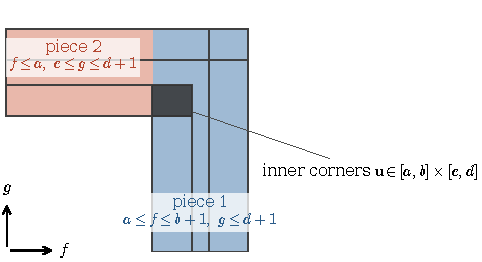
\includegraphics[width=0.62\textwidth]{figures/fig_boxunion.pdf}
\caption{\Cref{lem:boxunion}, drawn in the coordinates $(f,g)$ of the hallway: the union of the hallways $X_j(\bu)$ over all inner corners $\bu$ in the box $[a,b]\times[c,d]$ (dark) is the union of the two shaded convex pieces. Four of the hallways are outlined.}
\label{fig:boxunion}
\end{figure}

\needspace{6\baselineskip}
\begin{lem}\label{lem:boxunion}
Let $a<b$ and $c<d$. Then
\[
\bigcup_{\bu\in[a,b]\times[c,d]}X_j(\bu)\;=\;\widehat{X}_j\;:=\;\{a\le f_j\le b+1,\ g_j\le d+1\}\cup\{f_j\le a,\ c\le g_j\le d+1\}.
\]
\end{lem}

\begin{proof}
A point lies in the first arm of some $X_j(\bu)$ with $\bu\in[a,b]\times[c,d]$ if and only if $a\le f_j\le b+1$ and $g_j\le d+1$, and in the second arm of some such $X_j(\bu)$ if and only if $f_j\le b+1$ and $c\le g_j\le d+1$. The part of the second set with $f_j\ge a$ is contained in the first set.
\end{proof}

For a box $E=\prod_{j}\big([a_j,b_j]\times[c_j,d_j]\big)\subset E_0$ we define
\[
\Gamma(E)=\lamstar\Big(B_W\cap\bigcap_{j=1}^k\widehat{X}_j\Big),
\]
where $\widehat{X}_j$ is formed with $a_j,b_j,c_j,d_j$ as in \cref{lem:boxunion}. For every $\bw\in E$ we have $B_W\cap X(\bw)\subset B_W\cap\bigcap_j\widehat{X}_j$, and therefore
\begin{equation}\label{eq:Gammabound}
\sup_{\bw\in E}\lamstar\big(B_W\cap X(\bw)\big)\le\Gamma(E).
\end{equation}

\subsection{Evaluating \texorpdfstring{$\Gamma(E)$}{Gamma(E)} exactly}\label{sec:exact}

Each set $\widehat{X}_j$ is the union of two closed convex polygonal regions with disjoint interiors, and $B_W$ is a convex polygon. Intersecting $B_W$ with $\widehat{X}_1,\dots,\widehat{X}_k$ one at a time, and splitting every polygon into its intersections with the two pieces of $\widehat{X}_j$, we write $B_W\cap\bigcap_j\widehat{X}_j$ as a union of at most $2^k$ closed convex polygons $P_1,\dots,P_m$ with pairwise disjoint interiors.

To find the connected components, form the \emph{contact graph}: its vertices are the polygons $P_i$, and two of them are joined by an edge if they intersect. The union of the polygons in a connected component of this graph is connected, and unions coming from different components of the graph are disjoint closed sets. So the connected components of $B_W\cap\bigcap_j\widehat{X}_j$ correspond to the components of the contact graph, and the area of each is the sum of the areas of its polygons.

Some polygons may be degenerate, reduced to a segment or a point. They have no area but can connect two other polygons, so they must be kept: discarding them could split a component and make the computed value of $\Gamma(E)$ too small.

The computation is exact if all the numbers involved are rational. Suppose that every angle in $A\cup B$ has rational sine and cosine, that is, $\sin a=p/r$ and $\cos a=q/r$ for a Pythagorean triple $p^2+q^2=r^2$, as for $\arcsin(3/5)$; Kallus and Romik also used such angles \cite[Section~4 and Appendix]{kallusromik2018}. Then all the affine functions $f_j,g_j$ have rational coefficients. If $W$ is rational, the box $E_0$ and every box obtained from it by repeated bisection have rational endpoints. Every vertex of every polygon $P_i$ is then the intersection of two lines with rational coefficients, and every area is rational.

A box $E$ passes the test ``$\Gamma(E)\le T$'' as follows. If $\sum_i\lambda(P_i)\le T$, it passes, since every component has area at most the total. Otherwise the contact graph is computed, and $E$ passes if every component has area at most $T$.

\subsection{Certificates}

\begin{defn}\label{def:certificate}
Let $A$, $B$, $W$ be as in \cref{lem:box} and $T>0$. A \emph{certificate} for the inequality $G(A;B)\le T$ is a finite binary tree whose nodes are boxes in $\R^{2k}$, such that
\begin{enumerate}[label=(\alph*)]
\item the root is the box $E_0$ of \cref{lem:box};
\item the two children of every internal node are the two halves of its box, obtained by bisecting it at the midpoint of one coordinate interval;
\item every leaf $E$ satisfies $\Gamma(E)\le T$.
\end{enumerate}
\end{defn}

\begin{prop}\label{prop:certificate}
If a certificate for $G(A;B)\le T$ exists, then $G(A;B)\le T$.
\end{prop}

\begin{proof}
By induction on the tree, the leaves cover $E_0$. Every $\bw\in E_0$ lies in some leaf $E$, and then $\lamstar(B_W\cap X(\bw))\le\Gamma(E)\le T$ by \eqref{eq:Gammabound}. \Cref{lem:box} completes the proof.
\end{proof}

A certificate is stored as the list of its nodes in preorder. An internal node is recorded as the index of the coordinate that is bisected, and a leaf as the letter \texttt{L}. The boxes themselves are not stored: they are determined by $E_0$ and the sequence of bisections.

\subsection{Finding a certificate}\label{sec:search}

The certificate is produced by a separate search program. At each box it evaluates $\Gamma$ in double-precision floating-point arithmetic. If the value is below $T-10^{-7}$, the box becomes a leaf; otherwise it is bisected along its longest side. The margin $10^{-7}$, and the rule that nearly touching polygons count as touching, make it unlikely that floating-point errors produce a leaf that fails the exact test.

None of these choices affects correctness. A wrong decision by the search can only produce a leaf $E$ with $\Gamma(E)>T$, or a tree of the wrong shape, and the exact check rejects both. In \cite{kallusromik2018} a single program, in exact arithmetic throughout, does both the search and the certification. Separating the two lets the search use fast floating-point arithmetic and keeps the program that must be trusted small.

\section{The computation}\label{sec:computation}

Let $\alpha_1=\arcsin(3/5)\approx36.87\dg$ and $\alpha_2=\arcsin(4/5)\approx53.13\dg$, the two acute angles of the $3$--$4$--$5$ right triangle.

\begin{thm}\label{thm:computation}
$G(\{\alpha_1,\alpha_2\};\{\alpha_1,\alpha_2\})\le\Tmain$.
\end{thm}

The proof of \cref{thm:computation} is a certificate in the sense of \cref{def:certificate}, verified by computer; the rest of this section describes it. First we deduce the main theorem.

\begin{proof}[Proof of \cref{thm:main}]
Let $T=\Tmain$. Then $T>\sqrt2$, since $353^2=124{,}609>80{,}000=2\cdot200^2$. Moreover $\sin\delta_T=1/T=200/353<3/5$, because $1000<1059$. Since $\sin\alpha_1=\cos\alpha_2=3/5$, this gives $\delta_T<\alpha_1<\alpha_2<\gamma_T$. So $A=B=\{\alpha_1,\alpha_2\}$ satisfies the hypotheses of both \cref{thm:reduction2} and \cref{thm:reductionZ}, and together with \cref{thm:computation} they give $\lambda(S)\le\Tmain$ for every ambidextrous sofa $S$ and for every sofa $S$ that passes through $Z_D$ with $D\ge7$.
\end{proof}

The threshold $\Tmain$ is the smallest we tried for this relaxation; \cref{sec:limits} describes how the cost of the search grows as the threshold decreases. The certificates, the checkers, the search program and the Lean project are available in the repository \url{https://github.com/devinokeefe/ambidextrous-sofa-bounds}.

\subsection{The data}

There are four hallways, $L_{\alpha_1}$, $L_{\alpha_2}$, $\rho L_{\alpha_1}$ and $\rho L_{\alpha_2}$, so the parameter space has dimension $8$. As noted after \cref{lem:width}, $W_{\alpha_1}=W_{\alpha_2}=5$, and we take $W=5$ and $B_W=[0,5]\times[0,1]$. \Cref{tab:data} lists the affine functions $f_j,g_j$ of \eqref{eq:Xj} and the intervals $I_j,J_j$ of \cref{lem:box}. The mirrored hallways have the same intervals as the unmirrored ones, because $\rho$ maps $B_W$ to itself.

\begin{table}[h]
\centering
\caption{The four hallways in \cref{thm:computation}, the affine functions of \eqref{eq:Xj}, and the parameter intervals of \cref{lem:box} for $W=5$.}
\label{tab:data}
\renewcommand{\arraystretch}{1.25}
\begin{tabular}{@{}lllll@{}}
\toprule
Hallway & $f_j(x,y)$ & $g_j(x,y)$ & $I_j$ & $J_j$ \\
\midrule
$L_{\alpha_1}$ & $(4x+3y)/5$ & $(-3x+4y)/5$ & $[-1,\,23/5]$ & $[-4,\,4/5]$ \\
$L_{\alpha_2}$ & $(3x+4y)/5$ & $(-4x+3y)/5$ & $[-1,\,19/5]$ & $[-5,\,3/5]$ \\
$\rho L_{\alpha_1}$ & $(4x-3y+3)/5$ & $(-3x-4y+4)/5$ & $[-1,\,23/5]$ & $[-4,\,4/5]$ \\
$\rho L_{\alpha_2}$ & $(3x-4y+4)/5$ & $(-4x-3y+3)/5$ & $[-1,\,19/5]$ & $[-5,\,3/5]$ \\
\bottomrule
\end{tabular}
\end{table}

\subsection{The checkers}

The certificate for \cref{thm:computation} was checked by three programs that share no code: the \emph{Lean checker}, whose correctness is proved in Lean (\cref{sec:lean}), the \emph{C checker} and the \emph{Python checker}. Each checker rebuilds the box $E_0$ from \cref{lem:box}, walks through the certificate, and verifies that $\Gamma(E)\le T$ for every leaf $E$. The C and Python checkers read the four hallways and the threshold from a small text file; in the Lean checker the hallways are fixed in the source code. \Cref{tab:certificates} records the verification runs.

\begin{table}[h]
\centering
\caption{The two certificates and their verification. All three checkers accepted both certificates. Times are wall-clock times on a desktop computer with an Intel Core i9-14900K; the number of threads or processes used is given in parentheses.}
\label{tab:certificates}
\begin{tabular}{@{}lrr@{}}
\toprule
 & $G\le 9/5$ & $G\le\Tmain$ \\
\midrule
Leaves & $20{,}620{,}238$ & $436{,}160{,}442$ \\
Maximal depth of the tree & $62$ & $71$ \\
File size (uncompressed) & $82$ MB & $1.74$ GB \\
\midrule
\multicolumn{3}{@{}l}{\emph{Running times}} \\
Search (floating point) & $54$ s (4) & $1{,}111$ s (4) \\
Lean checker (verified) & $32$ s (30) & $776$ s (30) \\
C checker (exact integers) & $104$ s (4) & $1{,}267$ s (4) \\
Python checker (exact rationals) & $971$ s (16) & $20{,}207$ s (16) \\
\bottomrule
\end{tabular}
\end{table}

\emph{The Python checker} computes with exact rational numbers, using the FLINT library \cite{flint} through its Python interface \cite{pythonflint}, or Python's built-in rationals. It forms the polygons $P_i$ by clipping with the half-planes $f_j\le b_j+1$ and $g_j\le d_j+1$ and then splitting each polygon into its parts with $g_j\ge c_j$ and with $g_j\le c_j$, $f_j\ge a_j$. These two parts also make up $\widehat{X}_j$, divided differently from \cref{lem:boxunion}. It decides whether two polygons touch with exact point-in-polygon and segment-intersection tests.

\emph{The C checker} computes with integers only; every arithmetic operation on coordinates and areas is checked for overflow. It rescales the plane by a common denominator so that every vertex of every polygon has integer coordinates, uses the two pieces of \cref{lem:boxunion}, and decides whether two polygons touch by clipping one of them with the half-planes that define the other. It also checks that the tree is complete, that each angle is given by a Pythagorean triple, and that $W\ge\min_aW_a$, as \cref{lem:box} requires.



\section{Formal verification}\label{sec:lean}

We formalised both theorems in the Lean~4 proof assistant \cite{lean4}, using the Mathlib library \cite{mathlib2020}. For \cref{thm:hand} the result is a complete formal proof; for \cref{thm:main} it is a formal proof that a Lean function $\mathtt{checkCert}$ certifies the bound whenever it returns \texttt{true}, together with a run of that function, compiled to machine code, on the certificate file. The formalisation has about $5{,}000$ lines, of which about $900$ make up the checker. Formal proofs that include large computations have been given before, most notably for the Kepler conjecture \cite{hales2017flyspeck}; for the ordinary moving sofa problem, Baek's proof has been formalised in Lean \cite{cureton2026movingsofa,cao2026sofaformal}.

\needspace{8\baselineskip}
\subsection{Definitions and statements}\label{sec:leanstatements}

The formal statements use the definitions of the moving sofa problem in the Formal Conjectures project \cite{formalconjectures} and the definition of ambidextrous sofas proposed in \cite{fc_pr6424}. We copied these definitions without change, so that our statements can be compared with a specification written independently of this paper. The main ones are reproduced in \cref{app:data}.

\needspace{9\baselineskip}
The main formal results are the following, where \texttt{zSofaConstant D} is $\muZ(D)$:
\begin{alltt}\small
theorem ambidextrousSofaConstant_le_two_sqrt_two_sub_one :
    ambidextrousSofaConstant \(\le\) ENNReal.ofReal (2 * \(\sqrt{2}\) - 1)

theorem zSofaConstant_le_two_sqrt_two_sub_one \{D : \(\mathbb{R}\)\} (hD : 7 \(\le\) D) :
    zSofaConstant D \(\le\) ENNReal.ofReal (2 * \(\sqrt{2}\) - 1)

theorem ambidextrousSofaConstant_le_of_checkCert \{T : \(\mathbb{Q}\)\} (hT : 5/3 \(\le\) T)
    \{bytes : ByteArray\} (h : checkCert T bytes = true) :
    ambidextrousSofaConstant \(\le\) ENNReal.ofReal T
\end{alltt}
A fourth theorem, not displayed, is the analogue of the third for \texttt{zSofaConstant D} with $D\ge7$. The hypothesis $T\ge5/3$ gives $\delta_T\le\alpha_1$ and $\alpha_2\le\gamma_T$, as required in \cref{thm:reduction2,thm:reductionZ}. All four theorems depend only on the three standard axioms of Lean: propositional extensionality, choice, and the soundness of quotients.

The formal definitions differ from \cref{def:sofa} in two inessential ways. First, a motion is a continuous path $m\colon[0,1]\to E(2)$ in the group of all isometries of the plane, with $m(0)=\mathrm{id}$, rather than a pair of an orientation and a translation. Such a path consists of rotations followed by translations, because the determinant of the linear part of $m(t)$ is continuous with values in $\{\pm1\}$; this is the first lemma of the formalisation. Second, areas are Lebesgue measures with values in $[0,\infty]$. A set is ambidextrous if both it and its reflection in the line $y=\frac12$ are moving sofas, as in \cref{rem:definitions}(2). Formal Conjectures does not contain the Z-shaped corridor, which we defined in the same style.

\needspace{8\baselineskip}
\subsection{The verified checker}

The function $\mathtt{checkCert}$ reads the certificate as a byte string, walks through the tree in preorder, recomputes the boxes from $E_0$, and applies the test of \cref{sec:exact} to every leaf. It verifies the same inequality $\Gamma(E)\le T$ as the C checker, but is organised so that its correctness is easy to prove. Unverified code makes choices, such as how to cut a polygon into horizontal slices and how to group the polygons, and verified code checks conditions on these choices that imply the required bound.

The polygons $P_\sigma$, for $\sigma\in\{1,2\}^4$, are the intersections of $B_W$ with one of the two pieces of each $\widehat{X}_j$. Every boundary line other than $y=0$ and $y=1$ has a nonzero coefficient of $x$, so each $P_\sigma$ has the form $\{(x,y):0\le y\le1,\ \ell_i(y)\le x\le r_k(y)\text{ for all }i,k\}$ with affine functions $\ell_i$ and $r_k$. Suppose that $[0,1]$ is divided into intervals $[y_0,y_1]$, and that for each interval one lower bound $\ell$ and one upper bound $r$ are chosen. On such an interval the width of $P_\sigma$ at height $y$ is at most $\pos{r(y)-\ell(y)}$, a convex function of $y$, so
\[
\lambda(P_\sigma)\le\sum\frac{y_1-y_0}{2}\Big(\pos{r(y_0)-\ell(y_0)}+\pos{r(y_1)-\ell(y_1)}\Big).
\]
This holds for every subdivision and every choice of $\ell$ and $r$, so the code that makes these choices needs no proof. It takes the upper envelope of the $\ell_i$ and the lower envelope of the $r_k$, and splits $[0,1]$ at the breakpoints of these envelopes and at the zeros of the width; with these choices the bound equals $\lambda(P_\sigma)$.

Contact between polygons is handled in the same way. If $r(y_0)<\ell(y_0)$ and $r(y_1)<\ell(y_1)$ on every interval, then $P_\sigma$ is empty, and applying this to $P_\sigma\cap P_\tau$ proves that two polygons are disjoint. For the component test, unverified code sorts the polygons into groups. The checker then verifies that polygons in different groups are disjoint and that each group has total area at most $T$. This suffices, because a connected set contained in a finite union of pairwise disjoint closed sets lies in one of them.

The checker carries out these tests in integer arithmetic, with heights scaled so that all crossings of boundary lines lie at integer heights. If a range check needed for this encoding fails, the leaf is checked in rational arithmetic instead. Both versions are proved to agree with a common specification.

The remaining ingredients are \cref{lem:box}, the inclusion in \cref{lem:boxunion}, and the fact that the leaves of a tree obtained by repeated bisection cover its root. The subtrees are checked in parallel, which does not affect the proof, since in Lean's logic a parallel task has the same value as the corresponding sequential computation. The runs of the compiled checker are reported in \cref{tab:certificates}.

\subsection{What the proof relies on}\label{sec:trust}

The proof of \cref{thm:main} consists of the arguments of \cref{sec:definitions,sec:relaxations,sec:reduction,sec:method} and the verification of one certificate. It can be verified in two ways, which rely on different things.

\emph{Through the formalisation.} The formal proofs are checked by Lean's kernel, and the value $\mathtt{checkCert}\ T\ \mathit{bytes}=\mathtt{true}$ is obtained by running compiled code. This route relies on the kernel, the Lean compiler and runtime (including the C compiler that Lean uses), the few unverified lines of the program that read the file, parse $T$ and print the result, and the formal definitions in \texttt{SofaBounds/Defs.lean}, which should be compared with \cref{def:sofa,def:z} (the main ones are reproduced in \cref{app:data}). No other code needs to be trusted: the third theorem displayed in \cref{sec:leanstatements} holds for every byte string, so the certificate need not be trusted, and the hallway data are part of the verified program rather than an input.

\needspace{8\baselineskip}
\emph{By hand and with the C or Python checker.} Here the arguments of \cref{sec:definitions,sec:relaxations,sec:reduction,sec:method} are checked by hand, and the certificate by one of these two programs. This route relies on the program correctly implementing the test of \cref{def:certificate}, on its having been compiled or interpreted and run correctly, and on the four hallway entries that it reads being those of \cref{tab:data}. For the runs of the Python checker reported here, it also relies on FLINT and its Python interface, which did the rational arithmetic.

\section{Concluding remarks}\label{sec:remarks}

\subsection{How far can the method go?}\label{sec:limits}

A relaxation can never prove a bound below $\muR$. Romik's shape turns monotonically through every orientation between $0\dg$ and $90\dg$ in both turns, so for all finite $A,B\subset[0\dg,90\dg]$ it lies in an intersection of the kind used in \cref{def:G}, by \cref{lem:frame}, and \cref{lem:relax} gives $G(A;B)\ge\muR$.

For the relaxation of \cref{thm:computation}, the hallway positions taken by Romik's motions at the orientations $\alpha_1$ and $\alpha_2$ give a connected intersection of area $1.7229\ldots$ (\cref{fig:relax}(a)). A local search over the eight parameters, in floating-point arithmetic, found the larger configuration of \cref{fig:relax}(b). Rounded to four decimals, its parameters are $\bu_{\alpha_1}=\bv_{\alpha_1}=(0.1260,\,0.4425)$ and $\bu_{\alpha_2}=\bv_{\alpha_2}=(0.1322,\,0.5397)$. For these values the intersection in \eqref{eq:G} is connected and has area $29{,}092{,}957{,}301/16{,}800{,}000{,}000=1.73172\ldots$, as we checked in exact rational arithmetic with the routines of the Python checker. Hence $1.7317<G(\{\alpha_1,\alpha_2\};\{\alpha_1,\alpha_2\})\le\Tmain$, and the bound of \cref{thm:computation} cannot be pushed below $1.7317$.

\begin{figure}[h]
\centering
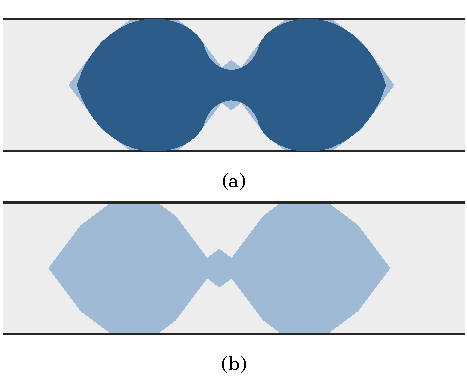
\includegraphics[width=0.66\textwidth]{figures/fig_relax.pdf}
\caption{The relaxation of \cref{thm:computation}. (a) Romik's shape $\Sigma$ (dark) inside the intersection of $H$ with the four hallways at the positions taken by Romik's motions at the orientations $\alpha_1$ and $\alpha_2$ (light); the intersection has area $1.7229\ldots$. (b) The configuration found by local search; the intersection has area $1.7317\ldots$. In both cases the intersection is connected.}
\label{fig:relax}
\end{figure}


\needspace{5\baselineskip}
The size of the certificate grows quickly as the threshold decreases (\cref{tab:growth}). No certificate exists for $T$ below the value of the relaxation, so one expects the number of nodes to grow without bound as $T$ decreases towards that value, or towards a somewhat larger one if the estimates on boxes are too weak.

\begin{table}[ht]
\centering
\caption{Size of the certificate for $G(\{\alpha_1,\alpha_2\};\{\alpha_1,\alpha_2\})\le T$ found by the search, for several thresholds $T$.}
\label{tab:growth}
\begin{tabular}{@{}lrrrrr@{}}
\toprule
$T$ & $1.85$ & $1.80$ & $1.78$ & $1.77$ & $1.765$ \\
\midrule
Nodes (millions) & $5.1$ & $41.2$ & $171.1$ & $475.2$ & $872.3$ \\
\bottomrule
\end{tabular}
\end{table}

Other choices of two angles on each side, including unequal sets $A\neq B$, gave local-search values between $1.732$ and $1.769$, no smaller than for $\{\alpha_1,\alpha_2\}$. Adding angles cannot increase the value of the relaxation, since $G(A';B')\le G(A;B)$ whenever $A\subset A'$ and $B\subset B'$, but it makes the search more expensive. With three angles on each side, for example $\{\alpha_1,\arcsin(119/169),\alpha_2\}$, local search finds configurations of area about $1.7217$, but at the threshold $1.85$ the search needed about six times as many nodes as with two angles.

Kallus and Romik proved that suitable maxima of their relaxations converge to the moving sofa constant as the angles become dense \cite[Theorem~5]{kallusromik2018}; the relaxations used there also constrain the final orientation of the sofa, by a set that contains all rotations of $V$ in a given range of angles. We have not proved the analogous statement for $G(A;B)$ and $\muA$. Even if it holds, our experiments suggest that two angles on each side will not give a bound much below $1.73$, and that more angles will be practical only with better estimates on each box or a reduction of the parameter space by symmetry.

\needspace{5\baselineskip}
\subsection{Open questions}

\begin{enumerate}[label=(\arabic*),leftmargin=*]
\item Is Romik's shape optimal? Is it at least locally optimal among nearby ambidextrous sofas? Romik lists local optimality as an open problem \cite{romik2018}. For numerical evidence and partial results see \cite{mohammed2026,bonfioli2026}.

\item Is $\muZ(D)$ equal to $\muA$ for all sufficiently large $D$?

\item Is $G(\{a\};\{a\})=\sec a+\csc a-\csc2a$ for all $a\in(0\dg,90\dg)$? At $a=45\dg$ this is \cref{prop:onehalf}. For $a=30\dg,35\dg,\dots,60\dg$, numerical local search from many random starting points reached this value to ten digits and never exceeded it. It would be the ambidextrous counterpart of the value $G_{(a)}=\sec a+\csc a$ for the ordinary problem \cite[Section~2]{kallusromik2018}.

\item Kallus and Romik showed that a moving sofa of maximal area must rotate by at least $81.2\dg$ \cite[Theorem~2]{kallusromik2018}. \Cref{prop:natural} shows that an ambidextrous sofa of area greater than $T$ rotates by at least $\gamma_T$ in each turn. Can the method of \cref{sec:method} show that ambidextrous sofas of area close to $\muA$ rotate substantially further?
\end{enumerate}


\appendix
\section{Proof of \texorpdfstring{Proposition~\ref*{prop:onehalf}}{Proposition 3.7}}\label{app:onehalf}

We integrate the lengths of horizontal slices. After a rotation of coordinates, we cover the intersection of the two hallways by two unit squares and two remaining regions, bound the length of each slice of these four sets, and so reduce \cref{prop:onehalf} to an inequality for a function of one variable (\cref{lem:Z}).

We compute areas in the coordinates
\[
p=\frac{x+y}{\sqrt2}, \qquad q=\frac{y-x}{\sqrt2},
\]
which are the coordinates $f_{45\dg}$ and $g_{45\dg}$ of \cref{sec:relaxations}. The change of coordinates is a rotation, so it preserves areas. The strip $H$ becomes the diagonal strip $\Delta=\{0\le p+q\le\sqrt2\}$. Throughout, $c=1/\sqrt2$ and $\psi(t)=\pos{1-|t|}$ denotes the tent function.

\subsection*{Slicing}
For $s\in\R$ consider the line $p+q=s$. For a set $E$ in the $(p,q)$-plane, let $m_E(s)$ be the length of the projection to the $p$-axis of the intersection of $E$ with this line. Since the map $(p,q)\mapsto(p,p+q)$ preserves area,
\begin{equation}\label{eq:slicing}
\lambda(E\cap\Delta)=\int_0^{\sqrt2}m_E(s)\,ds .
\end{equation}
For a unit square $U=[p',p'+1]\times[q',q'+1]$ one computes $m_U(s)=\psi(s-s_U)$, where $s_U=p'+q'+1$ is the value of $p+q$ at the centre of $U$.

\subsection*{A lemma on intervals}
\begin{lem}\label{lem:window}
Let $\phi\ge0$ be a continuous even function that is non-increasing in $|t|$. Among all intervals $I$ of a given length $\ell$, the integral $\int_I\phi$ is largest for $I=[-\ell/2,\ell/2]$.
\end{lem}

\begin{proof}
By symmetry we may take $I=[x-\ell/2,\,x+\ell/2]$ with $x\ge0$. The derivative of $\int_I\phi$ with respect to $x$ is $\phi(x+\ell/2)-\phi(x-\ell/2)\le0$, since $|x+\ell/2|\ge|x-\ell/2|$.
\end{proof}

In particular, a unit square $U$ as above satisfies $\lambda(U\cap\Delta)\le\int_{-c}^{c}\psi=\sqrt2-\frac12$.

\subsection*{The two hallways}
In the coordinates $(p,q)$, the hallway $L_{45\dg}(\bu)$ is
\[
\Lambda=\{p\le P_1,\ q\le Q_1\}\setminus\{p<P_1-1,\ q<Q_1-1\},\qquad P_1=u_1+1,\ Q_1=u_2+1 .
\]
A point $(x,y)$ lies in $\rho(L_{45\dg}(\bv))$ if and only if $(x,1-y)$ lies in $L_{45\dg}(\bv)$. Since $f_{45\dg}(x,1-y)=c-q$ and $g_{45\dg}(x,1-y)=c-p$, the mirrored hallway is
\[
\Lambda'=\{p\ge P_0,\ q\ge Q_0\}\setminus\{p>P_0+1,\ q>Q_0+1\},\qquad P_0=c-v_2-1,\ Q_0=c-v_1-1 .
\]
So both hallways are L-shaped regions with sides parallel to the axes, and their corners point in opposite directions.

\subsection*{A decomposition}
Let $R=[P_0,P_1]\times[Q_0,Q_1]$, and consider the four half-planes
\[
\mathrm{Rt}=\{p\ge P_1-1\},\quad \mathrm{Tp}=\{q\ge Q_1-1\},\quad \mathrm{Lf}=\{p\le P_0+1\},\quad \mathrm{Bt}=\{q\le Q_0+1\}.
\]
Within $R$ they consist of the points at distance at most $1$ from the right, top, left and bottom side of $R$, respectively. Then $\Lambda=\{p\le P_1,q\le Q_1\}\cap(\mathrm{Rt}\cup\mathrm{Tp})$ and $\Lambda'=\{p\ge P_0,q\ge Q_0\}\cap(\mathrm{Lf}\cup\mathrm{Bt})$, so
\[
\Lambda\cap\Lambda'=R\cap(\mathrm{Rt}\cup\mathrm{Tp})\cap(\mathrm{Lf}\cup\mathrm{Bt}).
\]
Expanding, $\Lambda\cap\Lambda'$ is the union of $R\cap\mathrm{Rt}\cap\mathrm{Bt}$, $R\cap\mathrm{Tp}\cap\mathrm{Lf}$, $R\cap\mathrm{Rt}\cap\mathrm{Lf}$ and $R\cap\mathrm{Tp}\cap\mathrm{Bt}$. The first two lie in the unit squares
\[
U_A=[P_1-1,P_1]\times[Q_0,Q_0+1], \qquad U_B=[P_0,P_0+1]\times[Q_1-1,Q_1].
\]
The part of $R\cap\mathrm{Rt}\cap\mathrm{Lf}$ inside $\mathrm{Tp}\cup\mathrm{Bt}$ lies in $U_A\cup U_B$, and likewise for the part of $R\cap\mathrm{Tp}\cap\mathrm{Bt}$ inside $\mathrm{Rt}\cup\mathrm{Lf}$. Hence
\[
\Lambda\cap\Lambda'\subset U_A\cup U_B\cup C_1\cup C_2,
\]
where $C_1=(R\cap\mathrm{Rt}\cap\mathrm{Lf})\setminus(\mathrm{Tp}\cup\mathrm{Bt})$ and $C_2=(R\cap\mathrm{Tp}\cap\mathrm{Bt})\setminus(\mathrm{Rt}\cup\mathrm{Lf})$.

\subsection*{Bounds on the slices}
Let $s_A=P_1+Q_0$ and $s_B=P_0+Q_1$ be the values of $p+q$ at the centres of $U_A$ and $U_B$, so that $m_{U_A}(s)=\psi(s-s_A)$ and $m_{U_B}(s)=\psi(s-s_B)$.

A point of $C_2$ has $P_0+1<p<P_1-1$ and $Q_1-1\le q\le Q_0+1$, with $q$ in an interval of length at most $1$. On the line $p+q=s$ the projections to the two axes have the same length. So the slice of $C_2$ has length at most $1$, at most $(s-Q_1+1)-(P_0+1)=s-s_B$, and at most $(P_1-1)-(s-Q_0-1)=s_A-s$. Thus
\[
m_{C_2}(s)\le\min\big(1,\ s-s_B,\ s_A-s\big)_+ ,
\]
and in the same way $m_{C_1}(s)\le\min(1,\ s-s_A,\ s_B-s)_+$. At most one of these two bounds is positive for any given $s$.

Let $s_0=(s_A+s_B)/2$, $\eta=|s_A-s_B|/2$ and $\xi=s-s_0$. Combining the bounds,
\begin{equation}\label{eq:mhat}
m_{\Lambda\cap\Lambda'}(s)\le\widehat m_\eta(\xi):=\psi(\xi-\eta)+\psi(\xi+\eta)+\min(1,\ \eta-|\xi|)_+ .
\end{equation}
By \eqref{eq:slicing}, $\lambda(\Lambda\cap\Lambda'\cap\Delta)\le\int_I\widehat m_\eta$, where $I=[-s_0,\sqrt2-s_0]$ is an interval of length $\sqrt2$. \Cref{prop:onehalf} therefore follows from the next lemma.

\begin{lem}\label{lem:Z}
For every $\eta\ge0$ and every interval $I$ of length $\sqrt2$,
\[
\int_I\widehat m_\eta\le2\sqrt2-1 .
\]
\end{lem}

\begin{proof}
The function $\widehat m_\eta$ is even, so it suffices to describe it for $\xi\ge0$. We distinguish three cases.

\emph{Case $\eta\ge1$.} For $0\le \xi\le\eta$ put $r=\eta-\xi\ge0$. Then $\psi(\xi+\eta)=0$ and
\[
\widehat m_\eta(\xi)=\pos{1-r}+\min(1,r)=1.
\]
For $\xi>\eta$, $\widehat m_\eta(\xi)=\psi(\xi-\eta)\le1$. So $\widehat m_\eta\le1$ and $\int_I\widehat m_\eta\le\sqrt2<2\sqrt2-1$.

\emph{Case $\tfrac12\le\eta\le1$.} For $0\le \xi\le\eta$ we get
\[
\widehat m_\eta(\xi)=(1-\eta+\xi)+\pos{1-\eta-\xi}+(\eta-\xi)=1+\pos{1-\eta-\xi}.
\]
For $\xi\ge\eta$ we have $\xi+\eta\ge1$, so $\widehat m_\eta(\xi)=\psi(\xi-\eta)\le1$. Hence $\widehat m_\eta(\xi)\le1+\pos{1-\eta-|\xi|}$ for all $\xi$, and
\[
\int_I\widehat m_\eta\le\sqrt2+(1-\eta)^2\le\sqrt2+\tfrac14<2\sqrt2-1 .
\]

\emph{Case $0\le\eta\le\tfrac12$.} Here, for $\xi\ge0$,
\[
\widehat m_\eta(\xi)=
\begin{cases}
2-\eta-\xi, & 0\le\xi\le\eta,\\
2-2\xi, & \eta\le\xi\le1-\eta,\\
1+\eta-\xi, & 1-\eta\le\xi\le1+\eta,\\
0, & \xi\ge1+\eta.
\end{cases}
\]
This function is continuous and non-increasing in $\xi\ge0$, so by \cref{lem:window}
\[
\int_I\widehat m_\eta\le\int_{-c}^{c}\widehat m_\eta .
\]
To compute the right-hand side, write $\widehat m_\eta(\xi)=2\psi(\xi)-\kappa(\xi)+\kappa(|\xi|-1)$ with $\kappa(t)=\pos{\eta-|t|}$, which one checks on each of the intervals above. Now $\int_{-c}^{c}2\psi=2\sqrt2-1$ and $\int_{-c}^{c}\kappa=\eta^2$, since $\eta\le\frac12<c$. The function $\kappa(|\xi|-1)$ is supported where $1-\eta\le|\xi|\le1+\eta$, and its integral over $[-c,c]$ is $\pos{\eta-(1-c)}^2$. Therefore
\[
\int_{-c}^{c}\widehat m_\eta=2\sqrt2-1-\eta^2+\pos{\eta-(1-c)}^2\le2\sqrt2-1,
\]
because $0<1-c$ implies $\pos{\eta-(1-c)}\le\eta$.
\end{proof}

\subsection*{The equality case}
Let $\bu=\bv=(0,c)$. Then $P_1=1$, $Q_1=1+c$, $P_0=-1$ and $Q_0=c-1$, so $U_A=[0,1]\times[c-1,c]$ and $U_B=[-1,0]\times[c,c+1]$. These squares share the corner $(p,q)=(0,c)$, which is the point $(x,y)=(-\frac12,\frac12)$. Here $s_A=s_B=c$, so $\eta=0$, and $C_1$ and $C_2$ are empty. The remaining parts $R\cap\mathrm{Rt}\cap\mathrm{Lf}$ and $R\cap\mathrm{Tp}\cap\mathrm{Bt}$ are the segments $\{0\}\times[c-1,c+1]$ and $[-1,1]\times\{c\}$, which lie in $U_A\cup U_B$. So $H\cap L_{45\dg}(\bu)\cap\rho(L_{45\dg}(\bv))$ corresponds to $(U_A\cup U_B)\cap\Delta$. This set is connected, because the two convex sets $U_A\cap\Delta$ and $U_B\cap\Delta$ share the point $(0,c)$. Its area is $2\int_{-c}^{c}\psi=2\sqrt2-1$ (\cref{fig:45}(b)). \qed

\section{The formal definitions}\label{app:data}

The formal statements of \cref{sec:leanstatements} rest on the definitions in \texttt{SofaBounds/Defs.lean}. The three below correspond to \cref{def:sofa}; like the hallways they use, they are copied from Formal Conjectures \cite{formalconjectures,fc_pr6424} and are shown without comments. Here \texttt{horizontalHallway}, \texttt{verticalHallway} and \texttt{hallway} are the sets $\Lh$, $\Lv$ and $L_0$ of \cref{sec:definitions}, $\mathbb{R}^2$ stands for \texttt{EuclideanSpace \(\mathbb{R}\) (Fin 2)}, \texttt{E(2)} is the group of isometries of $\R^2$ with its usual topology, \texttt{I} is the interval $[0,1]$, \texttt{m t \textquotesingle\textquotesingle{} s} is the image of \texttt{s} under \texttt{m t}, \texttt{midline} is the line $y=\frac12$, and \texttt{volume} is Lebesgue measure. The definitions for the Z-shaped corridor, which are ours, have the same form, with $Z_D$ in place of $L_0$.
\begin{alltt}\footnotesize
structure IsMovingSofa (s : Set \(\mathbb{R}\sp{2}\)) (m : I \(\to\) E(2)) : Prop where
  isConnected : IsConnected s
  isClosed : IsClosed s
  continuous : Continuous m
  zero : m 0 = .refl \(\mathbb{R}\) \(\mathbb{R}\sp{2}\)
  initial : s \(\subseteq\) horizontalHallway
  subset_hallway : \(\forall\) t, m t \textquotesingle\textquotesingle{} s \(\subseteq\) hallway
  final : m 1 \textquotesingle\textquotesingle{} s \(\subseteq\) verticalHallway
\end{alltt}
\needspace{5\baselineskip}
\begin{alltt}\footnotesize
def IsAmbidextrousSofa (s : Set \(\mathbb{R}\sp{2}\)) : Prop :=
  (\(\exists\) m, IsMovingSofa s m) \(\wedge\)
    (\(\exists\) m, IsMovingSofa (EuclideanGeometry.reflection midline \textquotesingle\textquotesingle{} s) m)
\end{alltt}
\needspace{4\baselineskip}
\begin{alltt}\footnotesize
def ambidextrousSofaConstant : \(\mathbb{R}{\ge}0\infty\) :=
  \(\bigsqcup\) (s : Set \(\mathbb{R}\sp{2}\)) (_ : IsAmbidextrousSofa s), volume s
\end{alltt}


\section*{Use of AI tools}
This work was carried out with significant help from Claude Opus~5.5 and GPT-6 Pro to develop and check the arguments of \cref{sec:reduction} and \cref{app:onehalf}, write the search program, the three checkers, and the Lean formalisation of \cref{sec:lean}, and write and review the paper. The author reviewed and edited the content as needed and takes full responsibility for the content of this paper.


\bibliographystyle{amsplain}
{\interlinepenalty=10000 % keep each reference on one page
\bibliography{references}}

\end{document}
